\chapter[Quantum States]{Quantum States}
\label{sec:2_quantum_states}


\chaptermark{Quantum States}

\rdv{2.1 has been cleaned up. 2.2 and 2.3 are still bad. 2.4 and 2.5 need more cleanup, but aren't too bad. n.b.: in the 12/19 draft, some figures and equations have moved and been renumbered.}

%\chapterauthor{Hein Mannaerts}

% \begin{abstract}
In this chapter, we will learn about quantum states: how to write them down, what they represent, and how they differ from classical states and bits.
Then, we will learn how to operate on and extract information from quantum states using unitary operations and measurements. Lastly, we'll discuss multiple quantum states and how to describe them.  Most of this chapter will be familiar to those who have taken an introductory quantum computing course.

% \end{abstract}

\section{Qubits}

% \subsection*{2.1.1: Qubits (Quantum bit)}

\rdv{term ket is introduced twice}

Recall from Chapter 1 that all information can be represented by classical bits in the classical world. Classical bits are confined to either the zero or one states, whereas the qubit can be "in-between" zero or one in  \textbf{superposition} states. Mathematically, the general qubit state for a superposition of $\ket{0}$ and $\ket{1}$ is represented using notation known as \textbf{Dirac Notation}, written
\begin{equation}
\ket{\psi} = \alpha \ket{0} + \beta\ket{1} 
\end{equation}
 where $\ket{\cdot}$ is pronounced \emph{ket}, $\psi$ (\emph{psi}) represents a general qubit state, $\alpha,\beta \in \mathbb{C}$.\label{def:ket}




First, let's discuss quantum bits, also known as \emph{qubits}. We have seen in the previous chapter that information can be represented by classical bits. In the classical world, a classical bit can only be in two states: it can be in a state we label \emph{zero}, or in a state we label \emph{one}, nothing in between. In contrast, a quantum bit can be anything in between. It can be 100\% zero or 100\% one, but it can also be 50\% zero and 50\% one or 1\% zero and 99\% one. Such a state is called a \emph{superposition} of zero and one. It's not that we don't know what the state is, it really is neither zero nor one but it's somewhere in between. (This notion of "in between" is not a completely accurate description, but it will do for now.  As we do the mathematics over the next several sections, your understanding will grow.)

% Dirac Notation w/ annotation
\begin{figure}[H]
    \centering
    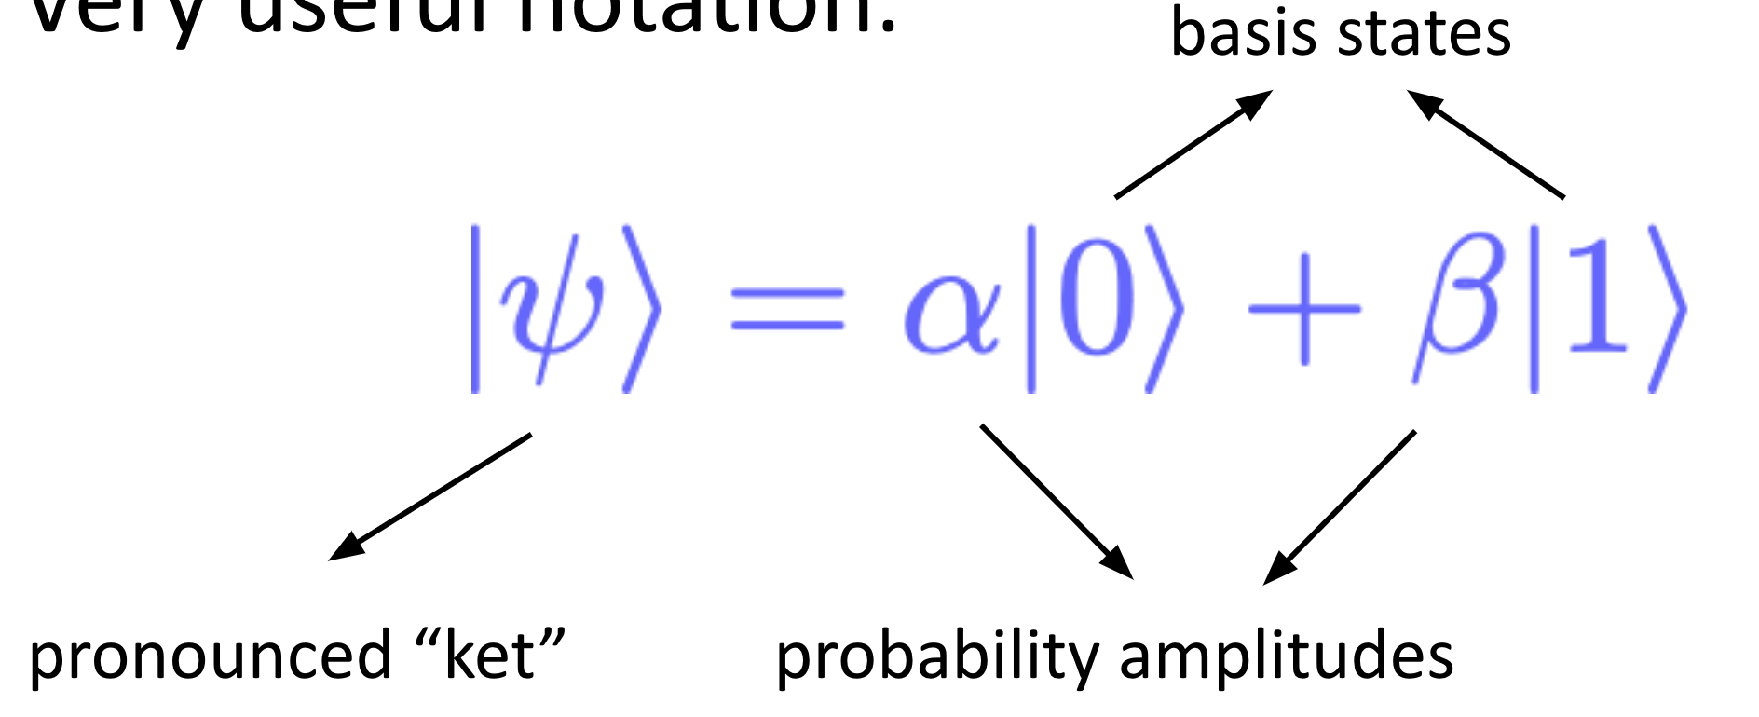
\includegraphics[width=0.8\textwidth]{lesson2/dirac_notation.pdf}
    
        \caption{Dirac ket notation. \rdv{This visual is probably helpful, needs to be redrawn or re-exported to get rid of that clipped text.}}
    
    \label{fig:ket-notation}
\end{figure}

The most common notation for writing down the state of a qubit (or more than one qubit) is called the \emph{Dirac notation}\index{Dirac notation}, and it's extremely useful. It's written like this,
\begin{align}
\ket{\psi} = \alpha\ket{0} + \beta\ket{1}
\end{align}
with this funny angle bracket \ket{}, pronounced \emph{ket}\index{ket}. The symbol $\psi$ (Greek letter "psi") in a ket, which we will call "state psi" or "ket psi" interchangeably, is often used to describe a general state of a qubit. $\ket{0}$ and $\ket{1}$ are called the \emph{basis states}\index{basis states}, and they determine what our state is. This $\alpha$ and $\beta$ are \emph{probability amplitudes}\index{probability amplitudes} that tell us how much of the state is in zero and how much of the state is in one.  These probability amplitudes can be any complex numbers, provided that they satisfy this normalization condition:
\begin{align}
    |\alpha|^2 + |\beta|^2 = 1
    \label{eq:normalization-condition}
\end{align}
(read "mod alpha squared plus mod beta squared is equal to one"). This is to ensure that whatever measurements we do in the future on this state produce results with the correct probabilities.


% Bloch Sphere
\begin{figure}[H]
    \centering
    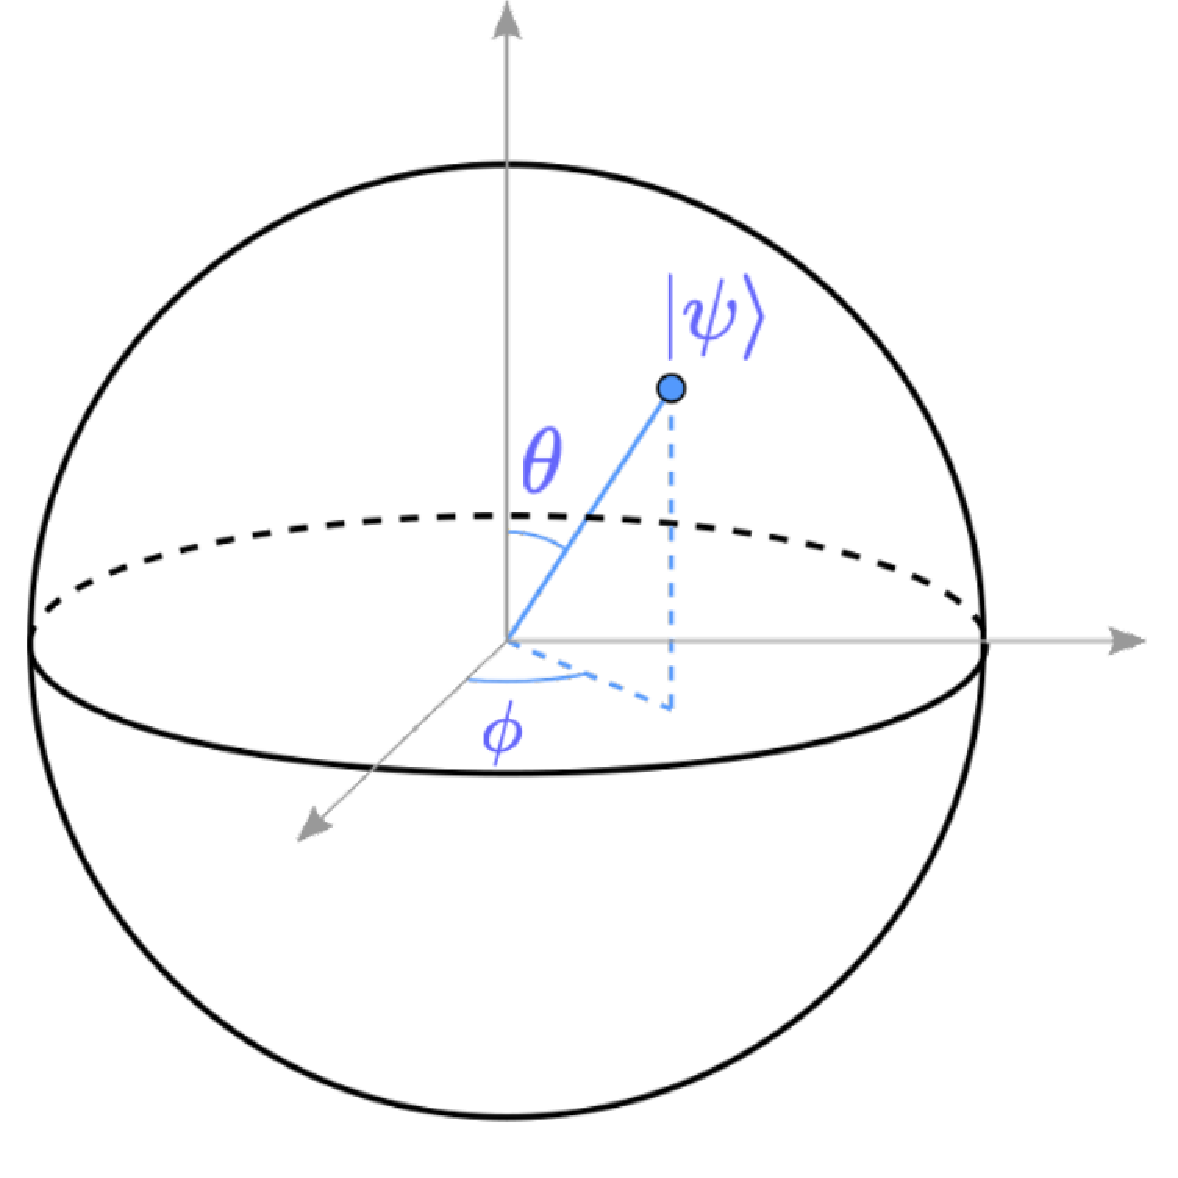
\includegraphics[width=0.6\textwidth]{lesson2/bloch_sphere.pdf}
    
        \caption{Bloch sphere}
    
    \label{fig:bloch}
\end{figure}

Another very useful representation of quantum states is using the \emph{Bloch sphere}\index{Bloch sphere}, as shown in Figs.~\ref{fig:bloch} and \ref{fig:annotated-bloch}. This visual representation gives us a very intuitive way of thinking about quantum states. All the states are given as points on the surface of the sphere, parameterized by the angle $\theta$ and the angle $\phi$. Then the state $\ket{\psi}$ can be written in the following form,
\begin{equation}
|\psi\rangle=\cos \frac{\theta}{2}|0\rangle+e^{i \phi} \sin \frac{\theta}{2}|1\rangle
\end{equation}
where the probability amplitude for basis state 0 is given by $\cos(\theta/2)$ and the probability amplitude for basis state 1 is given by $\sin(\theta/2)$, multiplied by $e^{i \phi}$, known as the complex phase of the state. This phase does not affect the probability of finding a one when we measure the qubit, but it is critically important as part of the state and in quantum algorithms.

This \ket{\psi} is a general state, but let's look at some examples, as in Fig.~\ref{fig:annotated-bloch}. We have already encountered \ket{0} and \ket{1}, and they sit at the north and the south pole of the Bloch sphere, respectively. We also said that we can have an arbitrary superposition of zero and one. For example, we can have a state known as the \emph{plus state}, written \ket{+}, which is an equal superposition of zero and one. The plus state appears on the equator of the Bloch sphere, at the point where the sphere's positive $X$ axis intersects the surface. We can have its friend the \emph{minus state}, written \ket{-}, on the other side of the Bloch sphere. It also is an equal superposition, but this time it's on the negative side of the $X$ axis.  It can be read "zero minus one", and if you think about a rotation about the $Z$ along the equator, since $e^{i\pi} = -1$, it has the complex phase $\pi$.  We can also have two states on the $Y$ axis. One is called the "plus i" state, written \ket{i} or occasionally \ket{+i}, and the other is called "minus i", written \ket{-i}. You can see that again, both of these states are an equal superposition of zero and one, but this time the phase between zero and one is given by the complex number $i$ or the angle $\pi/2$ for \ket{i} and $-i$ or the angle $3\pi/2$ for \ket{-}.  Summarizing, these states are
\begin{equation}
\begin{aligned}
& |\pm\rangle=\frac{1}{\sqrt{2}}(|0\rangle \pm|1\rangle) \\
& |\pm i\rangle=\frac{1}{\sqrt{2}}(|0\rangle \pm i|1\rangle).
\end{aligned}
\end{equation}

% insert Bloch sphere w/ axes labelled and |+> |-> meanings
\begin{figure}[H]
    \centering
    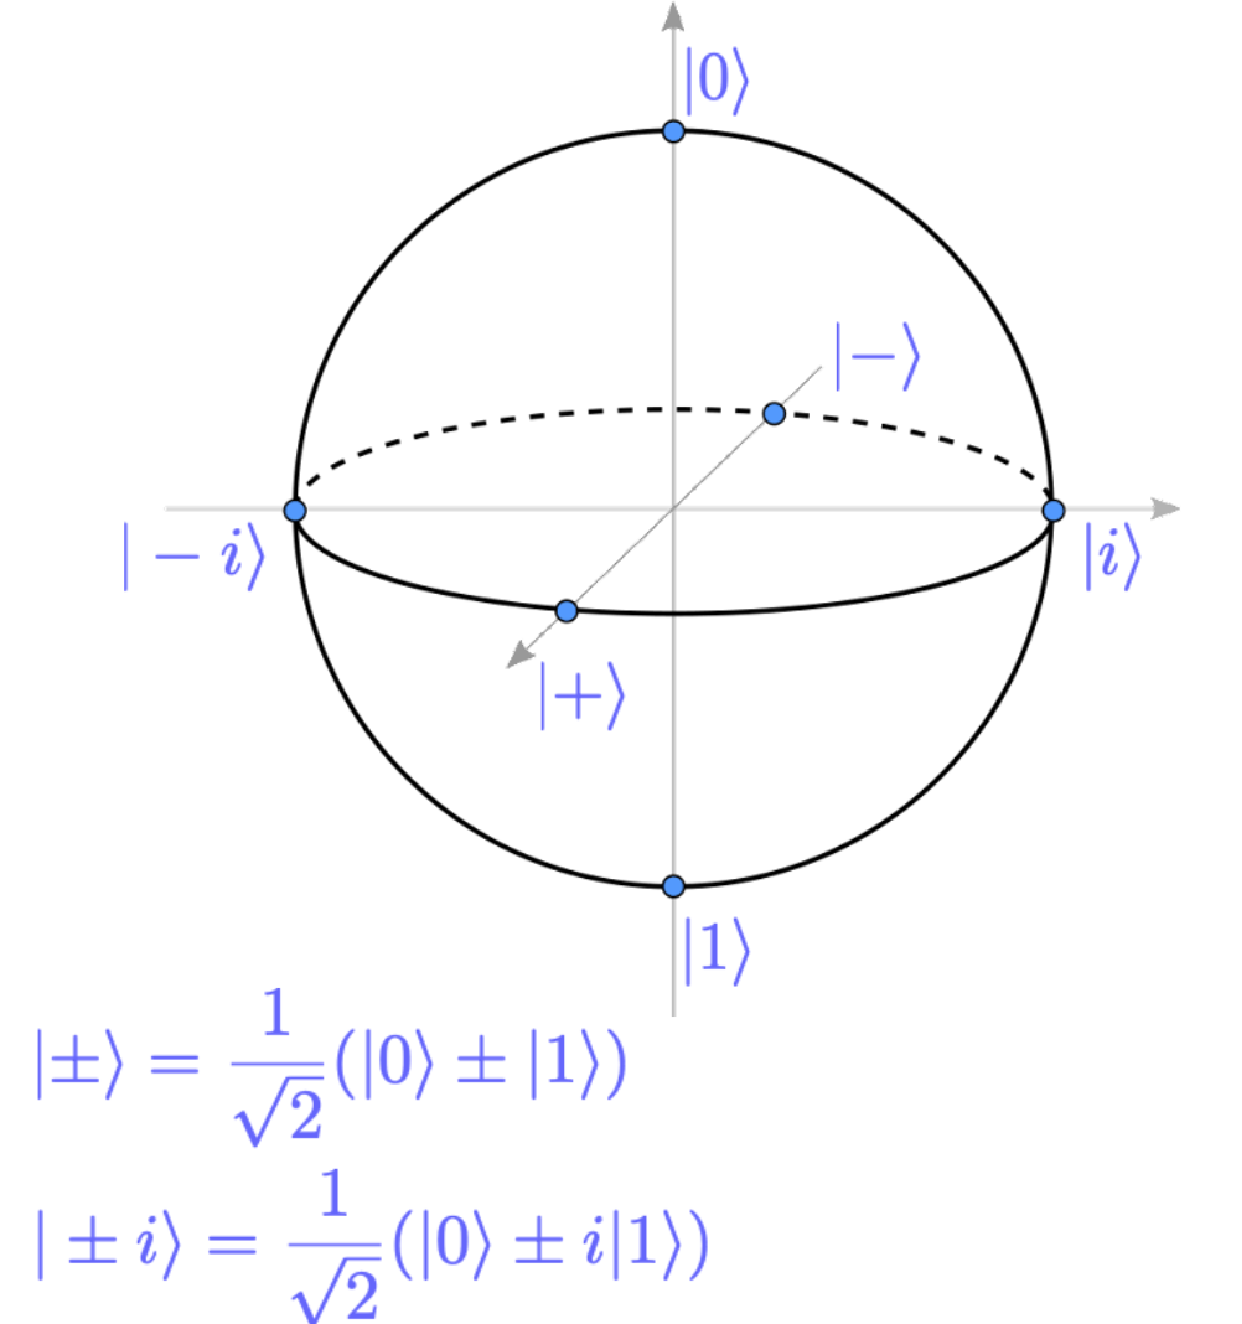
\includegraphics[width=0.7\textwidth]{lesson2/bloch_sphere_annotated.pdf}
    
        \caption{Bloch sphere with X, Y, and Z axis basis states.}
    
    \label{fig:annotated-bloch}
\end{figure}

\section{Unitary Operations}


% Classical (SSD) VS Quantum (Ion Trap)
\begin{figure}[H]
    \centering
    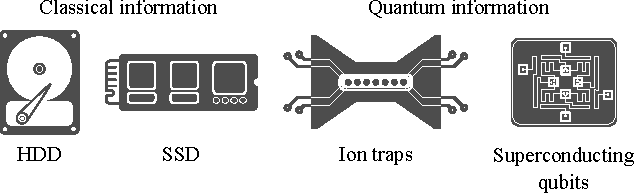
\includegraphics[width=0.9\textwidth]{lesson2/2-2_classical_quantum_info.pdf}
        \caption{A physical system.}
    \label{fig:physical-system}
\end{figure}

Let's see how we can manipulate quantum states, and therefore manipulate quantum information as well. We're going to do this with \emph{unitary operations}. One thing that you have to realize is that \emph{information is physical} (an aphorism coined by Rolf Landauer of IBM). This is because the information is represented by physical systems. Therefore, to change the information and process it, we have to interact with the physical systems that carry the information. In classical information, of course the primary processing technology is transistors manufactured using a photolithography process.  Computational states are represented using electrical charge, and information processing is done by using charge to control whether a switch is on or off, allowing charge to move from place to place within a computer chip.  Another very good example is HDDs (hard disk drives), where you read, write and manipulate information with very weak and precise magnetic fields. For an example of a younger technology, we can look at the "solid-state drive" where you do the same thing, but you achieve it by manipulating very weak electric currents.

In quantum information, on the other hand, we have physical systems such as \emph{ion traps}. For example, in a photo of an ion trap from a company called IonQ, individual atoms are represented by blue dots. The atoms are suspended on magnetic fields and they represent individual quantum bits. To manipulate the states of these qubits, you apply some laser pulses.  One of the most prominent forms of qubits is \emph{superconducting qubits} from companies such as IBM or Google, where microwave pulses manipulate the state of a quantum of electrical current. (Details of such processing hardware are beyond the scope of this module, but will be found in other modules in this series.) Some of these are represented in Fig.~\ref{fig:physical-system}.

But how do we actually describe these transformations? Before giving a more complete mathematical description, let's look at some examples, as shown in Fig.~\ref{fig:unitary-table}. The most simple transformation that we can think of is actually to do nothing, and we call this the \emph{identity operation}. It's usually represented by a capital $I$. When it's acting on a ket, it takes $\ket{0}$ to  $\ket{0}$  (written $\ket{0}\rightarrow\ket{0}$) and $\ket{1}$ to $\ket{1}$ ($\ket{1}\rightarrow\ket{1}$). Classically, we can also do something similar by just not touching our classical bit. 0 remains 0 and 1 remains 1.

% Simple Unitary Operations 
\begin{figure}[H]
    \centering
    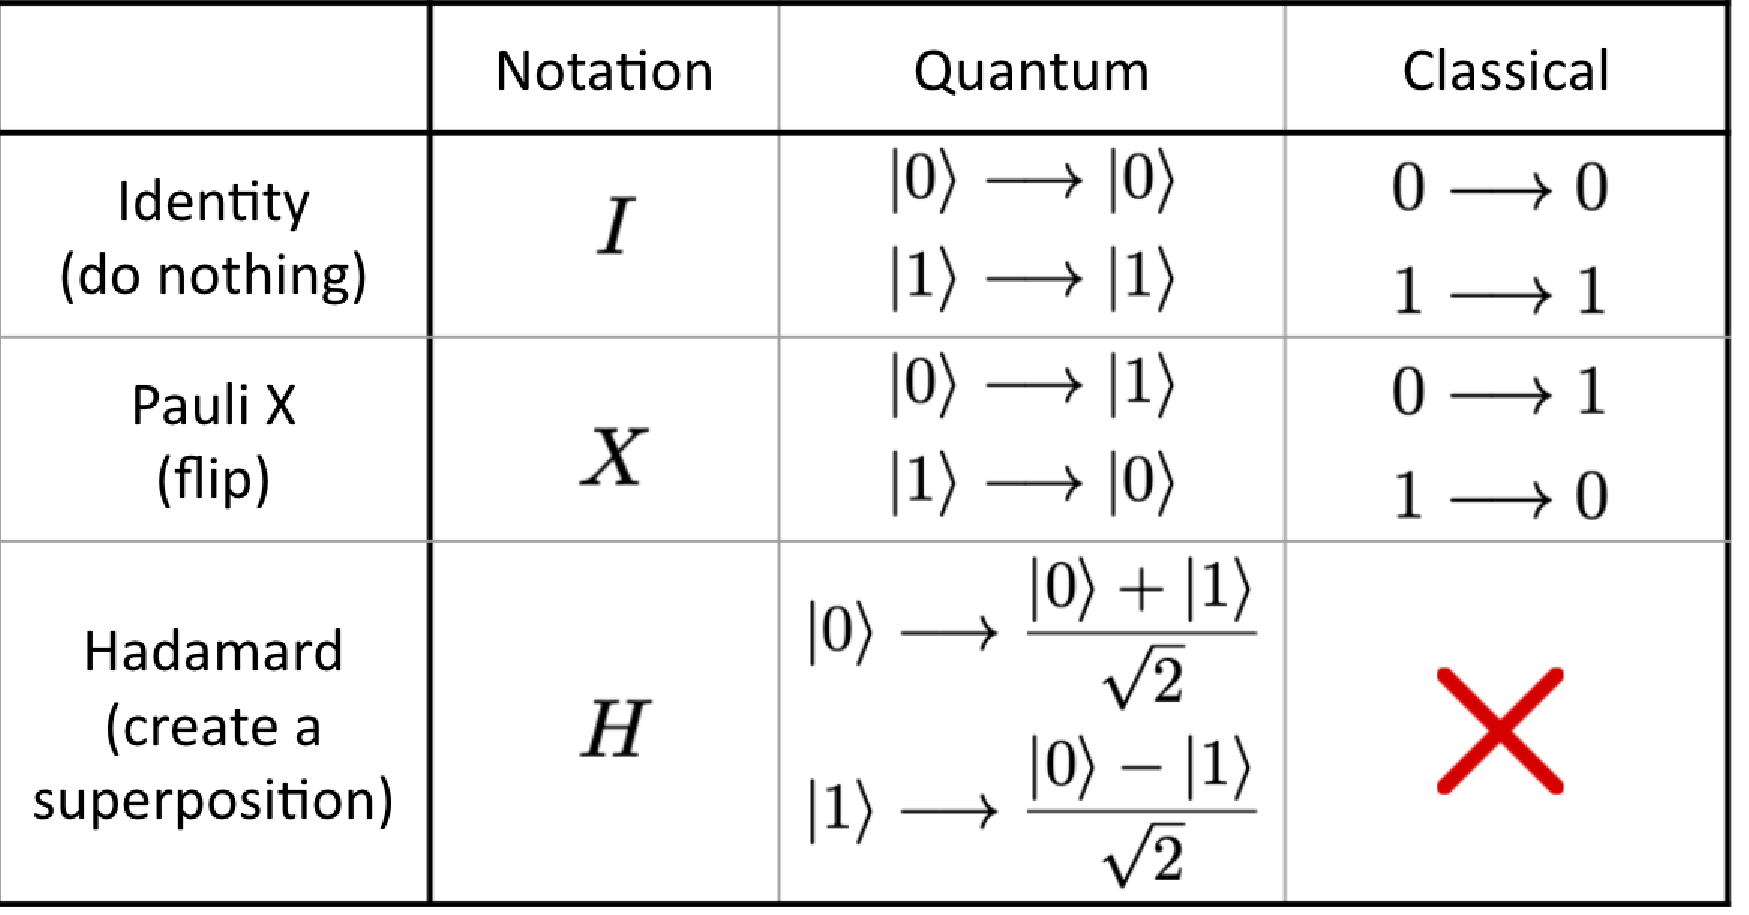
\includegraphics[width=0.7\textwidth]{lesson2/simple_unitary_ops.pdf}
    
        \caption{Simple unitary transforms. The bit flip has both a classical and a quantum form, but the Hadamard gate that creates a quantum superposition has no classical equivalent.}
    
    \label{fig:unitary-table}
\end{figure}

Another very simple operation is the \emph{flip}. Usually we call it either "flip" or a "Pauli X operation". We represent it by a capital $X$, and it does exactly what you would expect. It takes the input $\ket{0}$ into an output $\ket{1}$, and vice versa, $\ket{1}$ into a $\ket{0}$. Again, you have a corresponding classical operation as well, the NOT gate, which takes input 0 into classical bit 1 and input 1 into classical bit 0.

The third operation in Fig.~\ref{fig:unitary-table} creates superpositions. It is known as the \emph{Hadamard operator}\index{Hadamard}, denoted by $H$. If the input is $\ket{0}$, it outputs an equal superposition of \ket{0} and \ket{1}, written $(\ket{0}+\ket{1})/\sqrt{2}$. If the input is \ket{1}, the output will be $(\ket{0}-\ket{1})/\sqrt{2}$. This is the first example of a quantum operation that doesn't really have a classical analog, because we cannot have superpositions of classical bits.

So what's the definition of a unitary operation? All of these examples that we just discussed are examples of unitary operations. Any unitary operation has the property of being \emph{reversible}\index{reversible operation}, meaning we can undo its effect on our data and return to the original input state. This is done by what's known as an \emph{adjoint operator}\index{adjoint operator}, denoted as $U^\dagger$ (read "U dagger") where $U$ is the unitary.
Let's see how that works. We start with a ket $\ket{\psi}$ and we apply a unitary that transforms it into a completely new ket $\ket{\psi'}$. Then, if we apply the adjoint (the operation which undoes the effect of the original unitary), we end up back again at the state $\ket{\psi}$. We can write $\ket{\psi'} = U\ket{\psi}$, or we can also write $\ket{\psi} = U^\dagger\ket{\psi'}$. 

Let's put these two equalities together. Use the above equality for \ket{\psi}, then replace \ket{\psi'} with $U\ket{\psi}$ and get
\begin{equation}
|\psi\rangle=U^{\dagger}\left|\psi^{\prime}\right\rangle=U^{\dagger} U|\psi\rangle.
\end{equation} 

% We apply the $U^\dagger$, which is the same as applying the adjoint to the state $\ket{\psi'}$. But then again, we know the expression for $\ket{\psi'}$ from over here. So we can just substitute it in and we get $U^\dagger$ times U times the state $\ket{\psi}$, and that's it! You see that in order for these sides to be equal, we must conclude that $U^\dagger$ times U is the identity operator, and that makes logical sense. We are undoing the operation U with the adjoint, so the total effect of these two is we are doing nothing. Similarly, we can do it for $\ket{\psi'}$ which is equal to U applied to $\ket{\psi}$, and again we substitute for $\ket{\psi}$ this expression over here, and we get a similar expression as above: U times $U^\dagger$ times the state $\ket{\psi'}$. 

We can also do similar operations starting from the other expression and get
\begin{equation}
\left|\psi^{\prime}\right\rangle=U|\psi\rangle=U U^{\dagger}\left|\psi^{\prime}\right\rangle.
\end{equation}

From these equations,  we can see that also what needs to be true is that $UU^\dagger$ must be equal to the identity operator, and also $U^\dagger U$ must be equal to the identity.
% that's precisely the definition of unitary operations. There you go, that U times $U^\dagger$ must be equal to $U^\dagger$ times U, and that is equal to the identity. 
In fact, this becomes precisely our definition of a unitary operation: if $U$ satisfies the equation
\begin{equation}
U U^{\dagger}=U^{\dagger} U=I
\end{equation}
then it is unitary.

How can we represent this in matrix notation? So far we have been talking about states as kets, but in fact a ket is shorthand for a vector, and we know that in order to transform vectors we multiply them by matrices. Therefore, it should be the case that unitary operations can be represented by matrices. Let's look at some examples. 

First let's begin by seeing how kets for states become vectors. Usually we denote \ket{0} in vector notation as a column vector with 1 and 0,
\begin{equation}
\ket{0}\equiv\left(\begin{array}{l}
1 \\
0
\end{array}\right).
\end{equation}
The \ket{1}, on the other hand, is a column vector of 0 and 1,
\begin{equation}
\ket{1}\equiv\left(\begin{array}{l}
0 \\
1
\end{array}\right).
\end{equation}
You can see that any general state $\ket{\psi}$ can be represented as $\alpha$ times the vector $\left(\begin{array}{l}
1 \\
0
\end{array}\right)$ plus $\beta$ times $\left(\begin{array}{l}
0 \\
1
\end{array}\right)$, giving us the complex column vector $\left(\begin{array}{l}
\alpha \\
\beta
\end{array}\right)$. More formally, we have
\begin{equation}
\ket{\psi}=\alpha\left(\begin{array}{l}
1 \\
0
\end{array}\right)+\beta\left(\begin{array}{l}
0 \\
1
\end{array}\right)=\left(\begin{array}{l}
\alpha \\
\beta
\end{array}\right).
\end{equation}


Now let's look at examples of matrices representing unitary operations. The identity operator $I$ is represented by the matrix
\begin{equation}
I=\left(\begin{array}{ll}
1 & 0 \\
0 & 1
\end{array}\right).
\end{equation}
It's just a diagonal matrix with ones on the main diagonal and zeros everywhere else.

An important set of operations we will use many times is known as the set of \emph{Pauli operators}\index{Pauli operator}. We have encountered one Pauli operator already, the $X$ operator, which flips our ket from zero to one and from one to zero, but there are two other very important Pauli operators: the $Y$ and the $Z$. These three have the matrix representations 
\begin{equation}
\begin{aligned}
&X=\left(\begin{array}{ll}
0 & 1 \\
1 & 0
\end{array}\right) \\
&Y=\left(\begin{array}{cc}
0 & -i \\
i & 0
\end{array}\right) \\
&Z=\left(\begin{array}{cc}
1 & 0 \\
0 & -1
\end{array}\right)
\end{aligned}
\end{equation}

We also have the Hadamard operator~\footnote{In many physics books and papers, the symbol $H$ can also represent an operator known as the \emph{Hamiltonian} of a system.  In this book, we will not need the concept of the Hamiltonian. In general, it will be clear from context which one is meant.} that creates a superposition, written $H$.  The matrices corresponding to this operator is
\begin{equation}
H=\frac{1}{\sqrt{2}}\left(\begin{array}{cc}
1 & 1 \\
1 & -1
\end{array}\right).
\end{equation}


Let's see some examples just to give you a little bit of feeling for how this can actually work in practice. For the flip operation, you take the Pauli $X$, you apply it, or multiply it, by $\ket{0}$,
\begin{equation}
\begin{aligned}
X|0\rangle &=\left(\begin{array}{ll}
0 & 1 \\
1 & 0
\end{array}\right)\left(\begin{array}{l}
1 \\
0
\end{array}\right) \\
&=\left(\begin{array}{l}
0 \\
1
\end{array}\right)=|1\rangle.
\end{aligned}
\end{equation}

%So we see that 0 times 1 is 0, plus 1 times 0 is 0. So we get a 0 here in this first element of this new column vector, but then we have 1 times 1 plus 0 times 0 which is 1, and you see that this is actually our ket 1, so it indeed did flip a 0 into 1 as we would expect.

We can do the same thing for $\ket{1}$. Again, multiply the matrix representation of the Pauli $X$ operator with the column vector representation of state $\ket{1}$,
\begin{equation}
\begin{aligned}
X|1\rangle &=\left(\begin{array}{ll}
0 & 1 \\
1 & 0
\end{array}\right)\left(\begin{array}{l}
0 \\
1
\end{array}\right) \\
&=\left(\begin{array}{l}
1 \\
0
\end{array}\right)=|0\rangle
\end{aligned}
\end{equation}
and as expected we get $\ket{0}$. 

To create a superposition, take the Hadamard operator, apply it to the state $\ket{0}$. After going through the algebra, in the end we have an equal superposition of 0 and 1,
\begin{equation}
\begin{aligned}
H|0\rangle &=\frac{1}{\sqrt{2}}\left(\begin{array}{cc}
1 & 1 \\
1 & -1
\end{array}\right)\left(\begin{array}{l}
1 \\
0
\end{array}\right) \\
&=\frac{1}{\sqrt{2}}\left(\begin{array}{l}
1 \\
1
\end{array}\right)=\frac{1}{\sqrt{2}}(|0\rangle+|1\rangle)
\end{aligned}
\end{equation}

Please notice that this factor in the Hadamard operator, $1/\sqrt{2}$, ensures that the superposition vector at the end is properly normalized, as we saw in Eq.~\ref{eq:normalization-condition}. $|1/\sqrt{2}|^2 + |1/\sqrt{2}|^2 = 1$, therefore this vector is correctly normalized. You can follow the same process for the state 1, and again as we have seen in the previous step you get zero minus one,
\begin{equation}
\begin{aligned}
H|1\rangle &=\frac{1}{\sqrt{2}}\left(\begin{array}{cc}
1 & 1 \\
1 & -1
\end{array}\right)\left(\begin{array}{l}
0 \\
1
\end{array}\right) \\
&=\frac{1}{\sqrt{2}}\left(\begin{array}{c}
1 \\
-1
\end{array}\right)=\frac{1}{\sqrt{2}}(|0\rangle-|1\rangle).
\end{aligned}
\end{equation}
The modulus in Eq.~\ref{eq:normalization-condition} ensures that the negative coefficient still results in a non-negative probability and non-negative contribution to the normalization condition.

So far, the adjoint operator has been a rather abstract notion that can undo the effect of a unitary operation. How can we actually systematically find the adjoint 
of an operator, given the operator's unitary matrix? It's actually two very simple steps.
 
Step one: take the complex conjugate of the matrix. (Just to remind you, the \emph{complex conjugate}\index{complex conjugate} of a complex number $(x+iy)^*$ (read "x plus i y star"), which is the notation for complete conjugation, is
\begin{equation}
(x+i y)^{*}=x-i y
\end{equation}
Wherever you see $i$, flip the sign of that term to obtain the complex conjugate.)

Step two: take the transpose. The transpose of the matrix is given as follows: for any matrix $U$ which has elements $U_{00}$, $U_{01}$, $U_{10}$ and $U_{11}$, transposing them will exchange the off-diagonal elements. Let's see how this unitary $U$ actually turns into an adjoint. First we apply the complex conjugation, so we take each element and we write a little star, denoting that this element is complex conjugated, and then we apply the transpose,
\begin{equation}
U=\left(\begin{array}{ll}
U_{00} & U_{01} \\
U_{10} & U_{11}
\end{array}\right) \rightarrow\left(\begin{array}{cc}
U_{00}^{*} & U_{01}^{*} \\
U_{10}^{*} & U_{11}^{*}
\end{array}\right) \longrightarrow\left(\begin{array}{ll}
U_{00}^{*} & U_{10}^{*} \\
U_{01}^{*} & U_{11}^{*}
\end{array}\right)=U^{\dagger}
\end{equation}
We have flipped the position of the off-diagonal elements, but have not moved the diagonal elements. If you look at an example given by unitary Pauli $Y$ matrix written as this, first we take the complex conjugate so zero is just zero but the signs in front of these off-diagonal elements change because they're pure imaginary, and then we flip them because we're applying the transpose and we get the same matrix $Y$. When this happens, when the adjoint of a unitary matrix is equal to the unitary matrix, we say that that matrix is \emph{self-adjoint} and we will see many examples where this is, in fact, true.

\begin{equation}
Y=\left(\begin{array}{cc}
0 & -i \\
i & 0
\end{array}\right) \longrightarrow\left(\begin{array}{cc}
0 & i \\
-i & 0
\end{array}\right) \longrightarrow\left(\begin{array}{cc}
0 & -i \\
i & 0
\end{array}\right)=Y
\end{equation}

Another very important class of unitary operations are \emph{rotations}, and this is where the Bloch sphere representation will be extremely handy. The rotation can be written in this strange looking form (strange for now),

\begin{equation}
R_{\hat{n}}(\theta)=e^{-i \theta \hat{n} \cdot \hat{\sigma} / 2}
\end{equation}
and what it means is that we are rotating around some arbitrary direction in the Bloch sphere by some arbitrary angle $\theta$, and we write this as this following exponent. Here, $\hat{n}$ (read "n hat") is just a unit length vector given by coordinates $n_x$, $n_y$ and $n_z$, and the vector given by $\hat{\sigma}$ ("sigma hat") is just a vector of our Pauli matrices $X$, $Y$ and $Z$.  The dot product expands out to be
\begin{equation}
      \hat{n} \cdot \hat{\sigma} = n_{x} X+n_{y} Y+n_{z} Z
\end{equation}
and when put it in the equation we get
\begin{equation}
e^{-i \theta \hat{n} \cdot \hat{\sigma} / 2 }=\cos \frac{\theta}{2} I-i \sin \frac{\theta}{2}\left(n_{x} X+n_{y} Y+n_{z} Z\right).
\end{equation}
It does look a little bit complicated, but in the Bloch sphere representation it becomes very clear what's going on: take the vector $\hat{n}$ and rotate the state vector around that by the angle $\theta$. When we need this rotation, we can simply write it
\begin{equation}
R_{\hat{n}}(\theta)|\psi\rangle=\left|\psi^{\prime}\right\rangle.
\end{equation}

% So we can write this as follows: this exponential decomposes into cosine theta over 2 times the identity matrix minus i times sine theta 2, and then this expression which is just the dot product between these two vectors, so we multiply $n_x$ by Pauli matrix $X$, plus $n_y$ times Pauli matrix $Y$, plus $n_z$ times Pauli matrix $Z$. 



% insert Bloch sphere rotation y-axis
\begin{figure}[H]
    \centering
    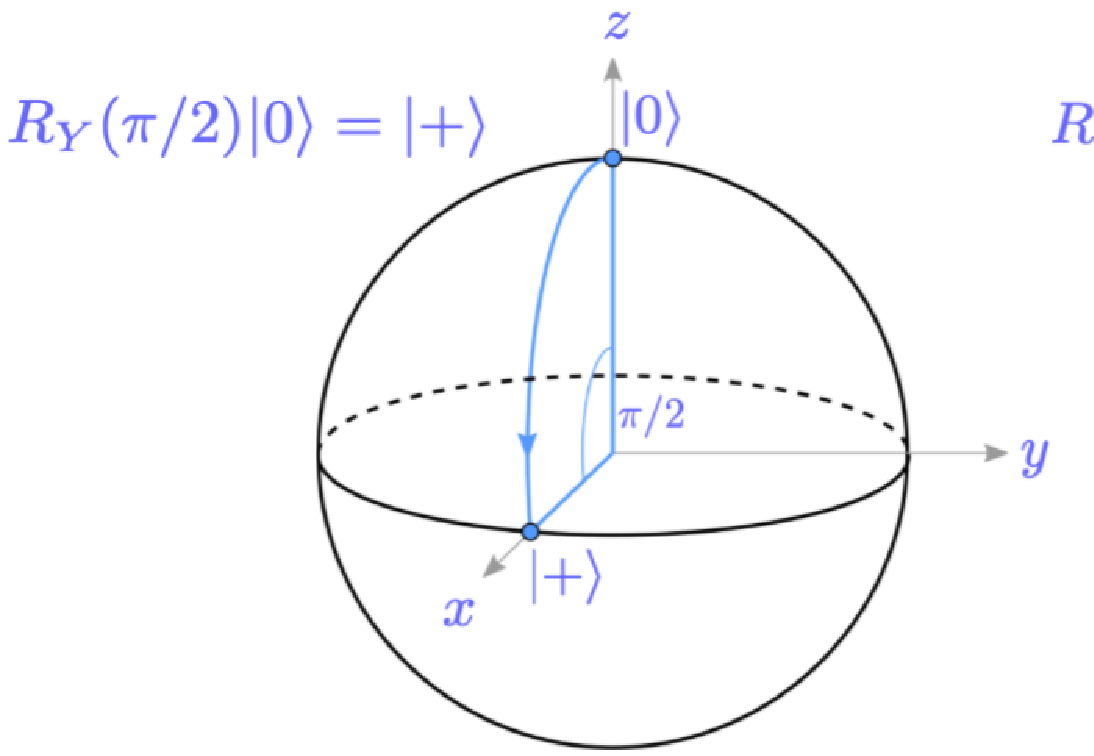
\includegraphics[width=0.7\textwidth]{lesson2/bloch_y_axis.pdf}
    
        \caption{Rotation about the Y axis}
    
    \label{fig:y-rot}
\end{figure}

Let's consider the example shown in Fig.~\ref{fig:y-rot}: we want to rotate around the y-axis through an angle of $\pi/2$, and our initial state is given by $\ket{0}$.  Let's start at the point $\ket{0}$, at the north pole of the sphere, and rotate around the y-axis. Going down along the surface by angle $\pi/2$, you see that we reach the state \ket{+}, which is an equal superposition of \ket{0} and \ket{1}.  For this $Y$ rotation, $\hat{n}$ simply becomes the unit vector along the positive y-axis, which we will just write $y$. Written out, we have
\begin{equation}
R_{y}(\pi / 2)\ket{0}=\ket{+}.
\end{equation}
(Be careful here; although this rotation took us from \ket{0} to \ket{+}, just like the Hadamard gate we have already seen, $H$ is not a $\pi/2$ $Y$ axis rotation.  Instead, $H$ is a $\pi$ rotation about the axis $(X+Z)/2$. See the exercises for more.)

\begin{figure}[H]
    \centering
    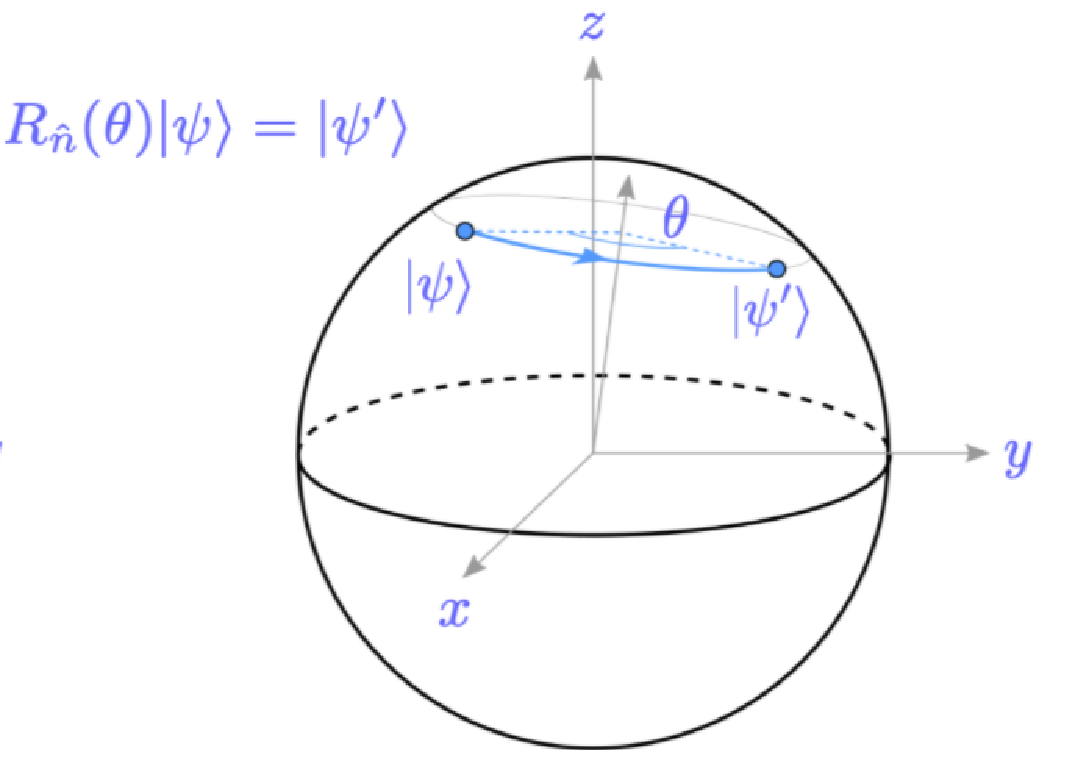
\includegraphics[width=0.7\textwidth]{lesson2/bloch_general_axis.pdf}
    
        \caption{Rotation about an arbitrary axis}
    
    \label{fig:arb-rot}
\end{figure}

More generally, it is not necessary to rotate about one of these orthogonal axes; you can rotate about any axis that you want, as in Fig.~\ref{fig:arb-rot}. You are rotating in the plane defined by your chosen axis and parameterized by the angle $\theta$. Take some initial state $\ket{\psi}$ that's on the surface of the Bloch sphere, follow the surface and end at some new state $\ket{\psi'}$.  (Note that the plane a particular state is rotating in does not have to pass through the center of the Bloch sphere, but the axis of rotation is normal to the plane.) 

So you can see that you can work in the matrix representation or you can work also in the Bloch sphere representation for single-qubit operations.


% $U_{00}$, $U_{01}$, $U_{10}$, $U_{11}$ 

\section{Measurement}
\label{sec:measurement}

\rdv{pick up editing here}

Now, let's consider measurements and how they can extract information from quantum qubits~\footnote{The type of measurements we consider in this book are \emph{projective measurements, as discussed more in the next chapter}. There are other types of measurement that you will learn about in advanced quantum classes.}. Basically a measurement asks the question: is my qubit in the state $\ket{0}$ or is it in the state $\ket{1}$? You can think of a measurement as a big box and you feed it your prepared state, as shown in Fig.~\ref{fig:z-measure}. Here, we consider a general state given by $\ket{\psi} = \alpha\ket{0}+\beta\ket{1}$, and the measurement operation tells you which state it is in. Usually there are only two possible values that can come out of a measurement device, which we will assign the values $+1$ and $-1$.

\begin{figure}[H]
    \centering
    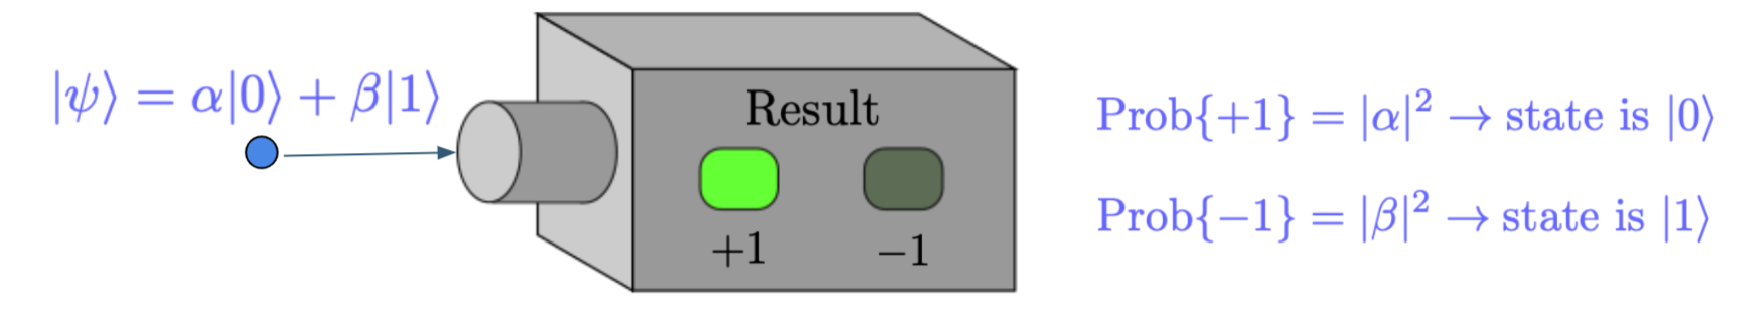
\includegraphics[width=0.7\textwidth]{lesson2/Pauli_z_machine.pdf}
    
        \caption{Measurement in the Z basis}
    
    \label{fig:z-measure}
\end{figure}

The probabilities of these measurement outcomes, corresponding to state \ket{0} and state \ket{1}, are given by their probability amplitudes. The probability of getting a $+1$ outcome is given by $|\alpha|^2$ and the probability of a $-1$ outcome is given by $|\beta|^2$. Immediately after the measurement, the state \emph{collapses} either onto \ket{0} or onto \ket{1}, so if you get a $+1$ outcome you can be sure that immediately after the measurement the state is in the state \ket{0}, or if you get a $-1$ then the state of the system has changed from the initial $\ket{\psi}$ and is \ket{1},
\begin{align}
\operatorname{Prob}\{+1\}=|\alpha|^2 \rightarrow \textrm{state is } |0\rangle \\
\operatorname{Prob}\{-1\}=|\beta|^2 \rightarrow \textrm{state is } |1\rangle.
\end{align}

\rdv{Michal, please check} (Mathematically speaking, the $\pm 1$ outcomes of the measurement are the \emph{eigenvalues} corresponding to the \emph{eigenvectors} of the Pauli $Z$ operator.  One way to remember which value corresponds to which vector is that $+1$ corresponds to \ket{0}, and $(-1)^0 = +1$, while $-1$ corresponds to \ket{1}, and $(-1)^1 = -1$.)

We refer to this particular measurement as a measurement in the \emph{computational basis} or in the Pauli $Z$ basis. This already hints at the fact that this is not the only measurement we can do. We can also ask the following question: is the state in the $\ket{+}$ state or in the $\ket{-}$ state? We can answer this question by rewriting our original state
\begin{equation}
|\psi\rangle=\alpha|0\rangle+\beta|1\rangle
\end{equation}
using the algebraic identities
\begin{equation}
|0\rangle=\frac{1}{\sqrt{2}}(|+\rangle+|-\rangle) \quad|1\rangle=\frac{1}{\sqrt{2}}(|+\rangle-|-\rangle).
\end{equation}
Notice that $\ket{0}$ is given by an equal superposition of the $\ket{+}$ state with the $\ket{-}$ state and the state $\ket{1}$ is \emph{also} an equal superposition of $\ket{+}$ and $\ket{-}$, but this time with a minus phase in front of the $\ket{-}$ state. We can rewrite our original state $\ket{\psi}$ in terms of these \ket{+} and \ket{-} states, but this time the probability amplitudes are
%for the state plus is $\alpha+\beta$ renormalized by the square root of two, and the probability amplitude for the minus state is $\alpha-\beta$,
\begin{equation}
\ket{\psi}=\frac{\alpha+\beta}{\sqrt{2}}\ket{+}+\frac{\alpha-\beta}{\sqrt{2}}\ket{-}.
\end{equation}
Again, we can feed our qubit into the measurement device and it will give us an answer $\ket{+}$ or $\ket{-}$ with the following probabilities,
\begin{align}
\label{eq:plus-measurement}
\operatorname{Prob}\{+1\}=\frac{|\alpha+\beta|^2}{2} \rightarrow \textrm{state is } |+\rangle \\
\label{eq:minus-measurement}
\operatorname{Prob}\{-1\}=\frac{|\alpha-\beta|^2}{2} \rightarrow \textrm{state is } |-\rangle.
\end{align}
You can see that the probabilities still depend on $\alpha$ and $\beta$, but they're not just $|\alpha|^2$ and $|\beta|^2$.
%they're in fact alpha plus beta the whole thing mod squared and alpha minus beta the whole thing squared and both of them are divided by two. 
Because we were asking a different question (whether the state state is in $\ket{+}$ or $\ket{-}$), the state changes from $\ket{\psi}$ and goes to $\ket{+}$ or $\ket{-}$ after the measurement, depending on the measurement outcome. This measurement is known as measurement in the Pauli $X$ basis.

In fact, you can measure in any basis that you can think of.  This is explored more in the exercises.

I've been using this word \emph{basis}, but what is a "basis"? Maybe you remember from your linear algebra class that the basis is a set of vectors that allows you to write down any vector that you can think of. In particular, if we have some general vector $\ket{\psi}$, we can write it in the Pauli Z basis given by $\ket{0}$ and \ket{1}, and already we have talked about the vector representations for $\ket{0}$ and one. And then the state in Dirac notation is written as follows, or you can write it in a new basis. Let's say you want to write it in terms of the states $\ket{i}$ and $\ket{-i}$. This is known as the Pauli $Y$ basis, and their vector representations are given as
\begin{align}
    |i\rangle=\frac{1}{\sqrt{2}}\left(\begin{array}{l}1 \\ i\end{array}\right) \quad|-i\rangle=\frac{1}{\sqrt{2}}\left(\begin{array}{c}1 \\ -i\end{array}\right).
\end{align}
%So it's just (1, i) and (1, -i) with the appropriate normalization factor in front, and 
Then the state can be rewritten as
\begin{equation}
|\psi\rangle=\frac{\alpha-i \beta}{\sqrt{2}}|i\rangle+\frac{\alpha+i \beta}{\sqrt{2}}|-i\rangle.
\end{equation}
These two vectors look very different but they represent the same state: the state has not changed, it's just that our description of the state is a little bit different because we have chosen a different basis in which to describe it.

Another very important concept is the \emph{inner product}\index{inner product}. The inner product is basically a dot product between two vectors, just as you probably learned in your basic linear algebra class, but to talk about it in our notation, first we have to define a \emph{bra}\index{bra}. Given a state $\ket{\psi}$, we can write down its bra, which is just its adjoint. So the bra of state $\ket{\psi}$ is given as the dagger of the original column vector,
\begin{equation}
\langle\psi|=(|\psi\rangle)^{\dagger}=\left(\begin{array}{l}
\alpha \\
\beta
\end{array}\right)^{\dagger}=\left(\begin{array}{ll}
\alpha^{*} & \beta^{*}
\end{array}\right).
\end{equation}
You apply the same trick as we applied for defining the adjoint of unitaries: you take the complex conjugate of $\alpha$ and $\beta$ and then you transpose the column vector, which turns it into a row vector. Now you can find the inner product between two arbitrary states, $\ket{\psi} = \alpha\ket{0} + \beta\ket{1}$ and $\ket{\phi} = \gamma\ket{0} + \delta\ket{1}$. Then we write it as 
%this: so we have bra times the ket in vector representation it's given by this. We have the row vector of
%(gamma star, delta star) multiplying the column vector (alpha, beta) and you get this following expression out:
\begin{equation}
\langle\phi \mid \psi\rangle=\left(\begin{array}{ll}
\gamma^{*} & \delta^{*}
\end{array}\right)\left(\begin{array}{c}
\alpha \\
\beta
\end{array}\right)=\alpha \gamma^{*}+\beta \delta^{*}.
\end{equation}
This should be no surprise if you remember your dot products from your linear linear algebra class.

Also notice that if you take the inner product of the state with itself, you in fact get this expression:
\begin{equation}
\langle\psi \mid \psi\rangle=|\alpha|^{2}+|\beta|^{2}=1
\end{equation}
Mod alpha squared plus mod beta squared will be equal to one, if the state is properly normalized. For two different states, you can also come across the scenario where the inner product between two states is zero,
\begin{equation}
\langle\phi \mid \psi\rangle=0.
\end{equation}
In that case, we say that the two states are \emph{orthogonal}.
%, just like in your classical linear algebra class between normal vectors.

How do we obtain these probabilities for the measurement outcomes? We have stated them as a fact before, but now you will see how to actually get them. We have our general state $\ket{\psi}$, and we say that we want to measure in some arbitrary basis $\ket{b_0}$ and $\ket{b_1}$. We are asking the question: is my state in the state $b_0$ or is my state in the state $b_1$? This is where the inner product comes in. We take the inner product between $\ket{b_0}$ and $\ket{\psi}$, we take the modulus and we square it, and that gives us the probability of a $+1$ outcome, and correspondingly the probability of the $-1$ outcome is given by the inner product between $\ket{b_1}$ and $\ket{\psi}$ modulus squared,
\begin{equation}
\begin{aligned}
\operatorname{Prob}\{+1\}&=\left|\left\langle b_{0}\mid \psi\right\rangle\right|^{2} \\
\operatorname{Prob}\{-1\}&=\left|\left\langle b_{1}\mid \psi\right\rangle\right|^{2}.
\end{aligned}
\end{equation}

To illustrate this with some simple examples, we're going to measure in the Pauli Z basis, and again, the probability of outcome one is given by mod alpha squared and probability of minus one is given by mod beta squared,
\begin{equation}
\begin{aligned}
\operatorname{Prob}\{+1\} &=|\langle 0 \mid \psi\rangle|^2 \\
&=|\alpha|^2 \\
\operatorname{Prob}\{-1\} &=|\langle 1 \mid \psi\rangle|^2 \\
&=|\beta|^2.
\end{aligned}
\end{equation}

How about measuring in our Pauli $Y$ basis? Again, the probability of $+1$ is given by
\begin{equation}
\begin{aligned}
\operatorname{Prob}\{+1\} &=|\langle i \mid \psi\rangle|^2 \\
&=\frac{|\alpha-i \beta|^2}{2} \\
\operatorname{Prob}\{-1\} &=|\langle-i \mid \psi\rangle|^2 \\
&=\frac{|\alpha+i \beta|^2}{2}.
\end{aligned}
\end{equation}

To summarize the measurement process, you start with some initial state written in some basis,
%here I have written it in the computational or in the Pauli Z basis, 
and then you say, okay I want to perform a measurement in a given basis described by these basis states $\ket{b_0}$ and $\ket{b_1}$. If my outcome is $+1$, which happens with the probability given by the inner product between the basis state with the original state modulus squared, then my post measurement state is given by $\ket{b_0}$. Or, if I get the $-1$ outcome, which happens with probability given by the inner product of $\ket{b_1}$ with the initial state $\ket{\psi}$ modulus squared, then my post measurement state is given by $\ket{b_1}$. But there is something very important to keep in mind: the measurement outcome is only $+1$ or $-1$. It does not give you any information about these probability amplitudes $\alpha$ and $\beta$. In the next section, we will see more about those probability amplitudes.


% と表示できます。1の状態だったらマイナスの状態には位相をつけるでしょう。
\begin{figure}[H]
    \centering
    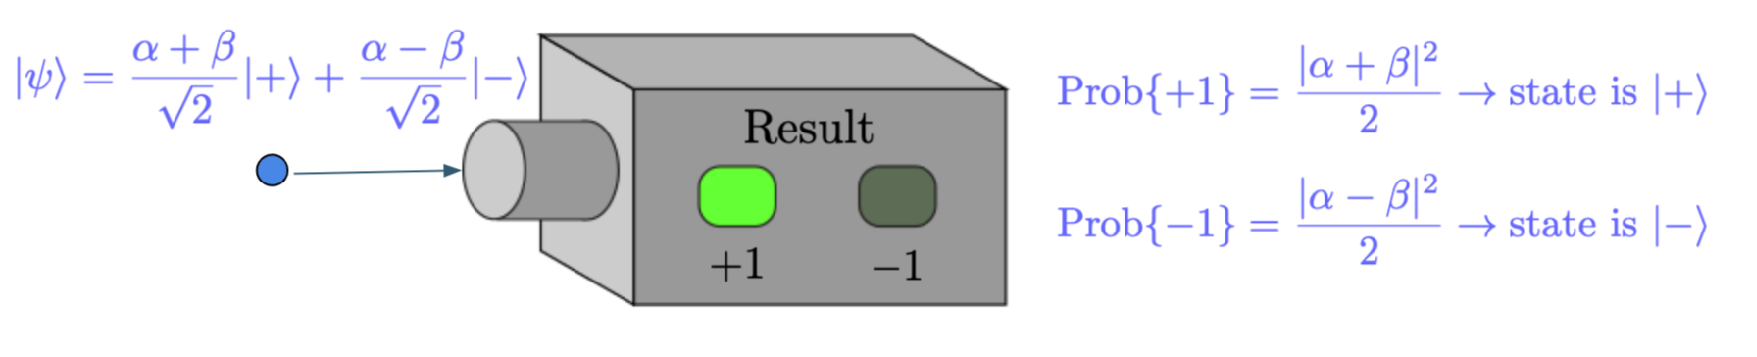
\includegraphics[width=0.7\textwidth]{lesson2/Pauli_x_machine.pdf}
    
        \caption{Measurement in the X basis}
    
    \label{fig:x-meas}
\end{figure}

% Insert basis representation pic here.
\begin{figure}[H]
    \centering
    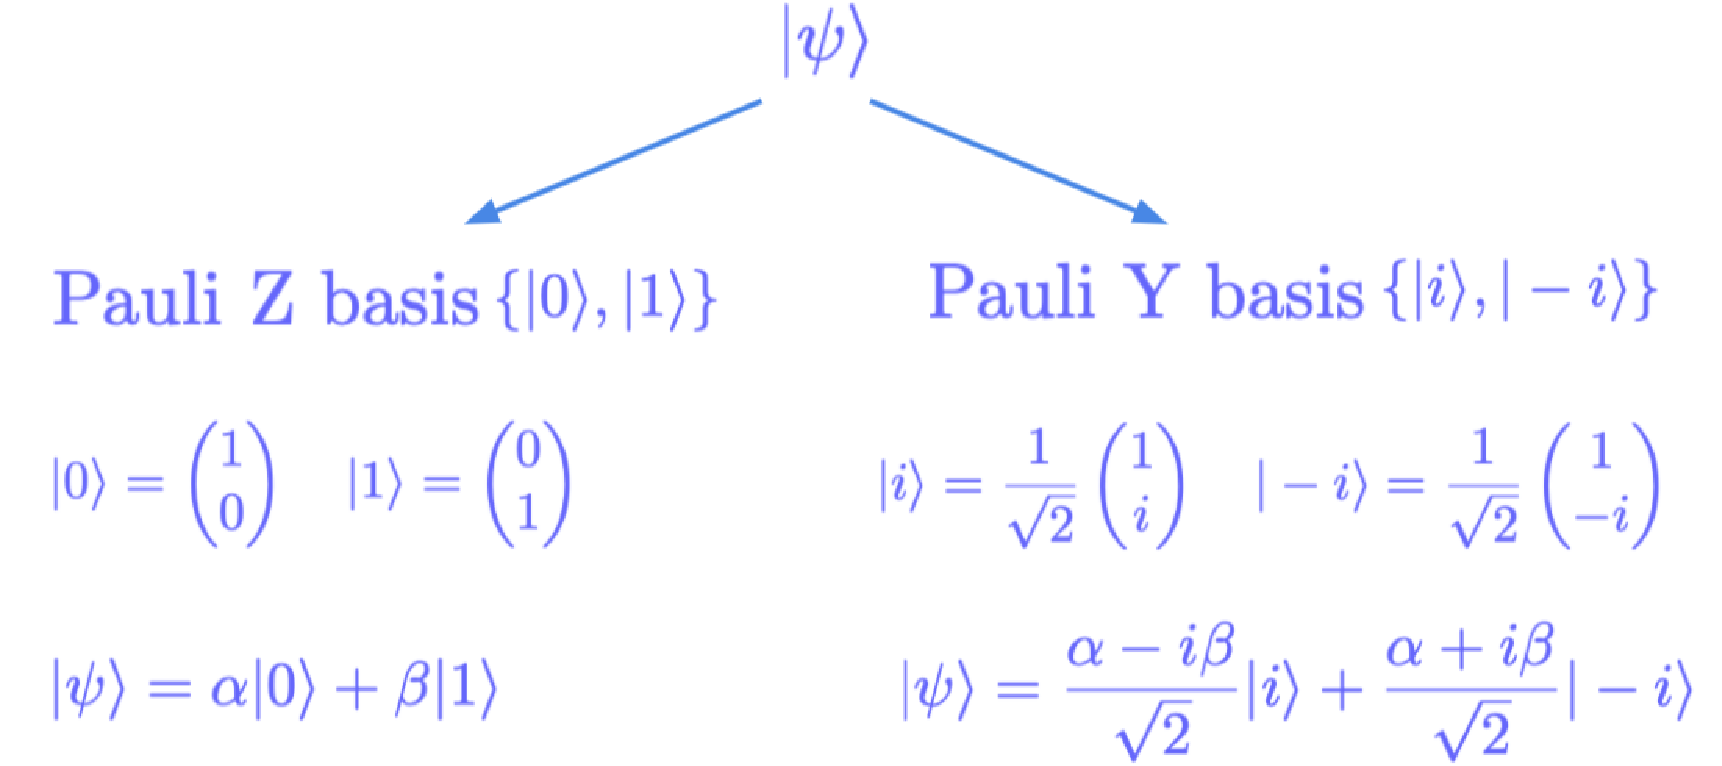
\includegraphics[width=0.7\textwidth]{lesson2/basis_representation.pdf}
    
        \caption{Basis state representation}
    
    \label{fig:bases}
\end{figure}

%%%%%%%%%%%%%%%%%%
\if0
\begin{figure}[H]
    \centering
    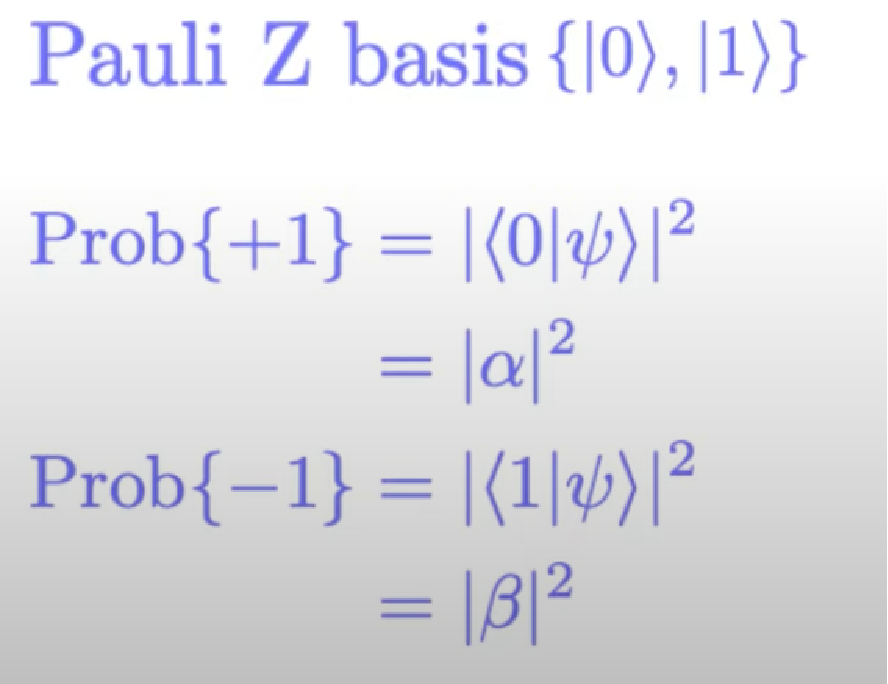
\includegraphics[width=0.5\textwidth]{lesson2/Pauli_z_ex.pdf}
    
        \caption{Probability in Z basis measurement}
    
    \label{fig: 1}
\end{figure}

% Pauli Y example
\begin{figure}[H]
    \centering
    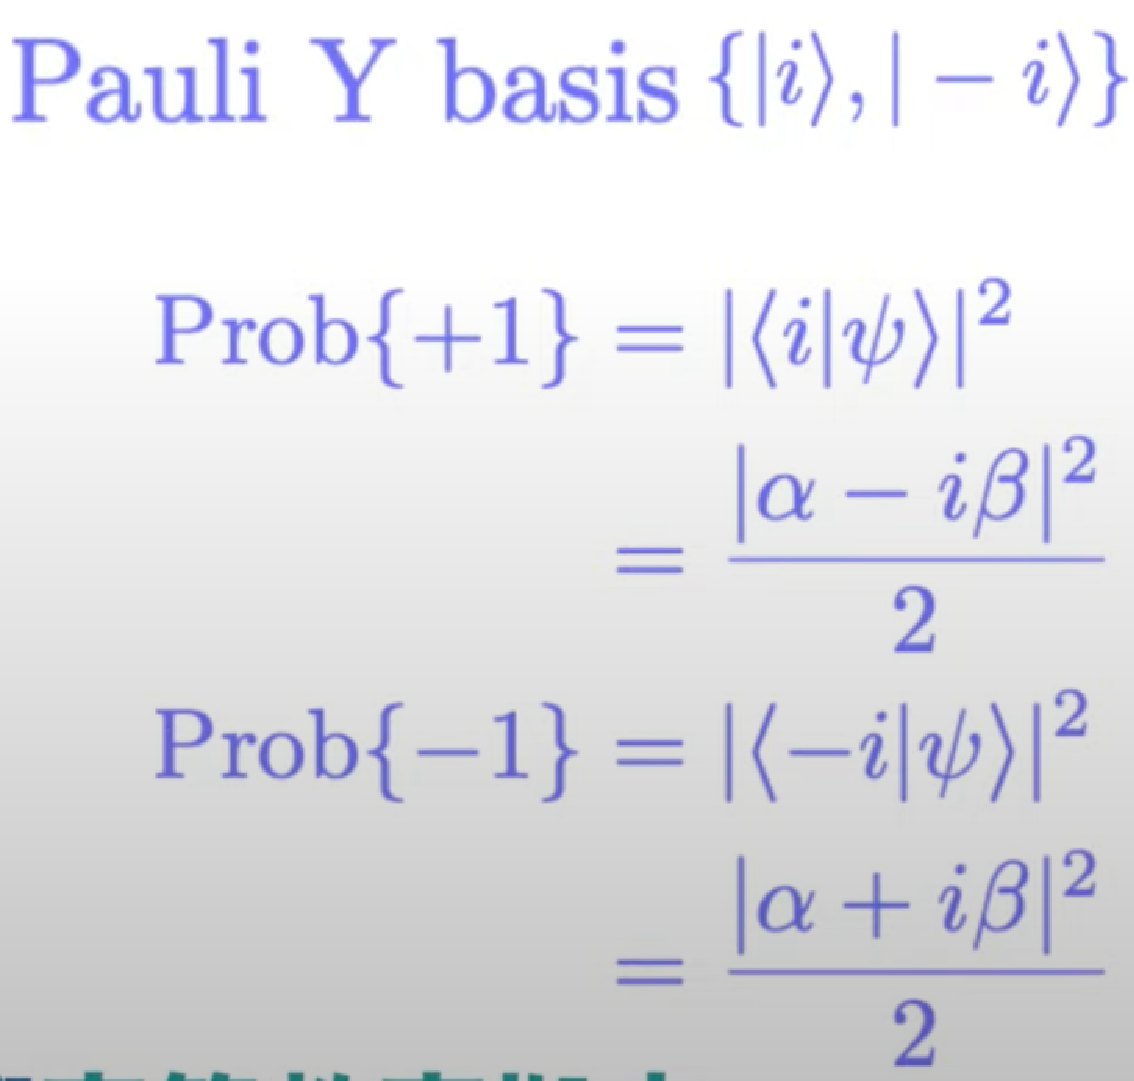
\includegraphics[width=0.5\textwidth]{lesson2/Pauli_y_ex.pdf}
    
        \caption{Probability in Y axis measurement}
    
    \label{fig: 1}
\end{figure}
\fi
%%%%%%%%%%%%%%%%%%

\section{Probabilities, expectation, variance}

We have seen how measurements can be applied to quantum states, but now let's see how we can actually extract information about the probabilities and the expectation values and variances of these measurements. Up to this point, we have only measured one single qubit as an individual event, as in Figs.~\ref{fig:z-measure} and \ref{fig:x-meas}.  This is known as \emph{single shot measurement}. Now let's consider the scenario where we have many copies of the same state and we keep measuring them again and again and again, as shown in Fig.~\ref{fig:many-copies}. We have our measurement device and we keep feeding it the same state: many copies of state $\ket{\psi}$. What comes out is a bit string of $+1$ and $-1$ results.

We can count the number of $+1$ outcomes, which we will denote by $N(+1)$, and we can count the number of $-1$ outcomes, which we will denote by $N(-1)$. Intuitively, the ratio between the number of $+1$ outcomes to the total number of measurements will be approximately equal to the probability of obtaining the plus one outcome, which is $|\alpha|^2$, and similarly for the fraction of the number of $-1$ outcomes, which will be very close to $|\beta|^2$,

\begin{equation}
\begin{aligned}
&\frac{N(+1)}{N(+1)+N(-1)} \approx|\alpha|^{2} \\
&\frac{N(-1)}{N(+1)+N(-1)} \approx|\beta|^{2}.
\end{aligned}
\end{equation}

In order to extract any information about the probabilities, we have to repeat the same measurement on a fresh copy of your state again and again and again. Because these measurements are random, we're not going to get the same answer every time. However, we can ask the question: what is the expected result when I measure in the Pauli Z basis? What number should I get if I repeat the same measurement many many times? Maybe you remember from your probability course that the \emph{expectation value} of some random variable is the sum of the probability of each possible outcome times its value. Let's call our variable $Z$ because we are measuring in the Pauli Z basis.  Its expectation value is given by the probability of the $+1$ outcome times $+1$ (the value of the outcome), plus the probability of $-1$ times the value of the outcome, which is in this case $-1$.  The probability of $+1$ remains $|\alpha|^2$, and the probability of the $-1$ outcome is given by $|\beta|^2$, but this time we are multiplying it by $-1$. So the expectation value when we measure in the Pauli Z basis is given by the expression
\begin{equation}
\begin{aligned}
\mathbb{E}[Z] &=\operatorname{Prob}(+1) \cdot(+1)+\operatorname{Prob}(-1) \cdot(-1) \\
&=|\alpha|^{2}-|\beta|^{2}.
\end{aligned}
\end{equation}

In Dirac notation, we write it as follows: we write the operator in which basis we are measuring and we enclose it in the angle brackets, but really it's just a shorthand for saying that we are multiplying the bra of state $\bra{\psi}$ times the $Z$ operator times the ket of state $\ket{\psi}$,

\begin{equation}
\langle Z\rangle=\langle\psi|Z| \psi\rangle.
\end{equation}

Let's check it: take the Pauli Z operator and sandwich it between our state given by the column vector $\alpha$ and $\beta$. Its bra is given by a row vector, so we have the row vector $\ket{\psi}$ times Pauli Z matrix times the column vector $\ket{\psi}$. When we multiply it out, we get the following expression which agrees with the expectation value that we have computed above.
\begin{equation}
\begin{aligned}
\langle Z\rangle &=\left(\begin{array}{ll}
\alpha^{*} & \beta^{*}
\end{array}\right)\left(\begin{array}{cc}
1 & 0 \\
0 & -1
\end{array}\right)\left(\begin{array}{l}
\alpha \\
\beta
\end{array}\right) \\
&=\left(\begin{array}{ll}
\alpha^{*} & \beta^{*}
\end{array}\right)\left(\begin{array}{c}
\alpha \\
-\beta
\end{array}\right) \\
&=|\alpha|^{2}-|\beta|^{2}
\end{aligned}
\label{eq:z-expectation}
\end{equation}

Again, because the number of the measurements are random we expect some degree of variance in our measurement outcomes, and again we use the same definition as from classical probability theory that the variance of some random variable is given by the expectation value of the square of that variable, minus the square of the expectation value of that variable,
\begin{equation}
\begin{aligned}
\operatorname{Var}[Z] &=\mathbb{E}\left[Z^{2}\right]-\mathbb{E}[Z]^{2}.    
\end{aligned}
\end{equation}
We have already computed the expectation value of Z, we don't need to do that anymore, we just square the expression from Eq.~\ref{eq:z-expectation}. Now we have to compute the expectation value of $Z^2$. That's the probability of getting a $+1$ outcome times $(+1)^2$ which is just $+1$.  The probability of the $-1$ outcome times $(-1)^2$, which is $1$, so actually what we get is
\begin{equation}
\begin{aligned}
\mathbb{E}\left[Z^{2}\right] &=\operatorname{Prob}\{+1\} \cdot(+1)^{2}+\operatorname{Prob}\{-1\} \cdot(-1)^{2} \\
&=|\alpha|^{2}+|\beta|^{2}.
\end{aligned}
\end{equation}

Often in physics you will see that the variance is referred to as \emph{fluctuations}, and that's denoted by $(\Delta Z)^2$ and that's really just the variance of Z. In the Dirac notation, we again have this expression,
\begin{equation}
\begin{aligned}
(\Delta Z)^{2} & \equiv \operatorname{Var}[Z] \\
&=\left\langle Z^{2}\right\rangle-\langle Z\rangle^{2}.
\end{aligned}
\end{equation}


% many copies machine
\begin{figure}[H]
    \centering
    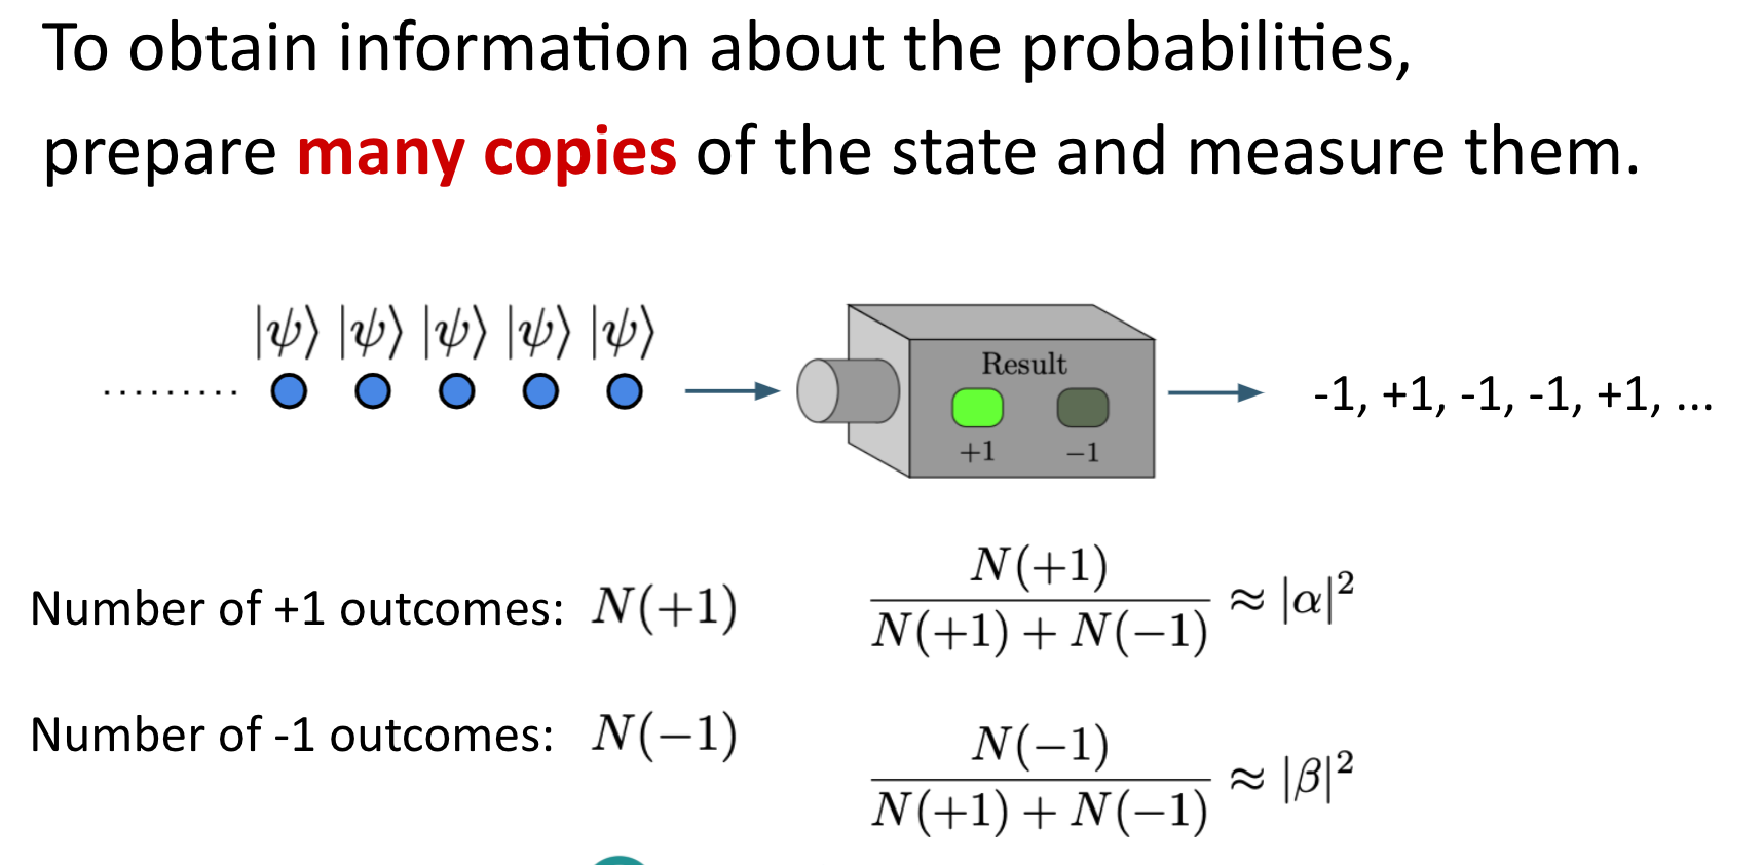
\includegraphics[width=0.5\textwidth]{lesson2/many_copies_machine.pdf}
    
        \caption{Repeated measurements}
    
    \label{fig:many-copies}
\end{figure}


\section{Multiple Qubits}
\label{sec:multi-qubit}

Now, let's consider how to write down the state of multiple qubits. So how do we write down the state of two bits? Let's start with a very simple question like that. Well, if we have two classical bits, they can be in four different states. They can be in $00$, $01$, $10$, or $11$. So what's the case for quantum bits? We need to switch to the Dirac notation. We can have the $\ket{00}$, $\ket{01}$, $\ket{10}$, and $\ket{11}$. Any general state of two qubits can be written as a superposition of these four states weighted by some probability amplitudes. We need four of them because we have four different states: $\alpha$, $\beta$, $\gamma$ and $\delta$, 
\begin{equation}
|\psi\rangle=\alpha|00\rangle+\beta|01\rangle+\gamma|10\rangle+\delta|11\rangle
\end{equation}
and again the state must be normalized such that when we measure, it gives the correct probabilities. But this time the normalization condition is as follows: it's mod of all the probability amplitude squared, when you sum it up it has to be equal to one again,
\begin{equation}
|\alpha|^2+|\beta|^2+|\gamma|^2+|\delta|^2 = 1.
\end{equation}
And again in vector notation, we can write these kets as follows: $\ket{00}$ now is a column vector of four elements: (one, zero, zero, zero), and similarly for $\ket{01}$, $\ket{10}$, and $\ket{11}$,
\begin{equation}
|00\rangle=\left(\begin{array}{l}
1 \\
0 \\
0 \\
0
\end{array}\right),|01\rangle=\left(\begin{array}{l}
0 \\
1 \\
0 \\
0
\end{array}\right),|10\rangle=\left(\begin{array}{l}
0 \\
0 \\
1 \\
0
\end{array}\right),|11\rangle=\left(\begin{array}{l}
0 \\
0 \\
0 \\
1
\end{array}\right).
\end{equation}
So you see that this is a nice orthogonal basis with which we can express any general state $\ket{\psi}$. In fact, we can now write our combination of those amplitudes above as a vector,
\begin{equation}
\ket{\psi}=\alpha\left(\begin{array}{l}
1 \\
0 \\
0 \\
0
\end{array}\right) + \beta\left(\begin{array}{l}
0 \\
1 \\
0 \\
0
\end{array}\right)+\gamma\left(\begin{array}{l}
0 \\
0 \\
1 \\
0
\end{array}\right)+\delta\left(\begin{array}{l}
0 \\
0 \\
0 \\
1
\end{array}\right)=\left(\begin{array}{l}
\alpha \\
\beta \\
\gamma \\
\delta
\end{array}\right).
\end{equation}

The very important mathematical concept behind being able to write the basis states like that is that of a \emph{tensor product}\index{tensor product}~\footnote{There are actually multiple types of tensor products; by one definition, a tensor is like an $n$-dimensional matrix instead of the customary two-dimensional one.  In this book, we will use tensors in a fashion that expands the vector or matrix size, instead of making it into a multidimensional object.}.

So how do we actually get these two new qubit basis states? We took some state of the first qubit, let's call it "a" because it can be anything, and we took a tensor product with another qubit state "b". Mathematically, you have a column vector for the first qubit given by these probability amplitudes $a_1$ and $a_2$ tensor product the column vector for the second qubit $b_1$ $b_2$, and this operation of the tensor product is defined as follows:

\begin{equation}
|a\rangle \otimes|b\rangle=\left(\begin{array}{l}
a_{1} \\
a_{2}
\end{array}\right) \otimes\left(\begin{array}{l}
b_{1} \\
b_{2}
\end{array}\right) \equiv\left(\begin{array}{l}
a_{1}\left(\begin{array}{l}
b_{1} \\
b_{2}
\end{array}\right) \\
a_{2}\left(\begin{array}{l}
b_{1} \\
b_{2}
\end{array}\right)
\end{array}\right)=\left(\begin{array}{l}
a_{1} b_{1} \\
a_{1} b_{2} \\
a_{2} b_{1} \\
a_{2} b_{2}
\end{array}\right)
\end{equation}

\if0
$
\left(\begin{array}{l}
a_1 \\
a_2
\end{array}\right)$
%のベクトルと
$\left(\begin{array}{l}
b_1 \\
b_2
\end{array}\right)$
\fi

To calculate the product, take the first probability amplitude $a_1$ times the whole column vector for $\ket{b}$. That will give you the first two elements in your new four dimensional vector.  $a_1$ times $b_1$ goes into the first entry in the resulting vector, $a_1$ times $b_2$ goes in the second entry, and then for the bottom two elements you take $a_2$ and again you multiply the whole column vector of $\ket{b}$, so you have $a_2$ times $b_1$ and $a_2$ times $b_2$.

In ket notation, we have $\ket{a} \otimes \ket{b}$, which can be represented in vector form. For example, if we have two qubits and the first qubit is in state $\ket{0}$ and the second qubit is in state one, we write it as column vectors and take the tensor product like this,
%(1 0) tensor product (0 1), and you can see that one times zero is zero, one times one is one, zero times zero is zero, and finally zero times one is zero,
\begin{equation}
|0\rangle \otimes|1\rangle=\left(\begin{array}{l}
1 \\
0
\end{array}\right) \otimes\left(\begin{array}{l}
0 \\
1
\end{array}\right)=\left(\begin{array}{l}
0 \\
1 \\
0 \\
0
\end{array}\right).
\end{equation}

Similarly, we can take the tensor product of more complicated states: we have tensor product of $\ket{1}$ with $\ket{-}$,
%so we have the column vector (0 1) tensor product this superposition with an extra minus phase in here, so it's one over square root of two, times the column vector one minus one, and that gives us this two-qubit state (0, 0, 1, -1), all renormalized by this one over square root of two,
\begin{equation}
|1\rangle \otimes|-\rangle=\left(\begin{array}{l}
0 \\
1
\end{array}\right) \otimes \frac{1}{\sqrt{2}}\left(\begin{array}{c}
1 \\
-1
\end{array}\right)=\frac{1}{\sqrt{2}}\left(\begin{array}{c}
0 \\
0 \\
1 \\
-1
\end{array}\right).
\end{equation}

The tensor product is very general; if you have two vectors with $m$ and $n$ entries, their tensor product will be a vector with $mn$ entries in it. When dealing with qubits, our vectors will generally have a length that is a power of two; each qubit you add to the system doubles the number of entries in the vector when we take the tensor product.

Also, for our purposes, the length of each individual vector is normalized, and the tensor product retains this property.

Finally, be careful: just as with ordinary matrix products, the order of vectors (kets) written in a tensor product matters. This will be explored in detail in the exercises.

How do we actually apply tensor products to matrices so that we can describe operations on multiple qubits? It's a very similar logic: we have two matrices "A" and "B", we take the tensor product between them. We take the first element $A_{11}$ of the first matrix and we multiply the entire second matrix by that value. This will give us the upper left region of the new four by four matrix. 

\begin{equation}
\begin{aligned}
A \otimes B &=\left(\begin{array}{ll}
A_{11} & A_{12} \\
A_{21} & A_{22}
\end{array}\right) \otimes\left(\begin{array}{ll}
B_{11} & B_{12} \\
B_{21} & B_{22}
\end{array}\right) \\
&=\left(\begin{array}{lll}
A_{11}\left(\begin{array}{ll}
B_{11} & B_{12} \\
B_{21} & B_{22}
\end{array}\right) & A_{12}\left(\begin{array}{ll}
B_{11} & B_{12} \\
B_{21} & B_{22}
\end{array}\right) \\
A_{21}\left(\begin{array}{ll}
B_{11} & B_{12} \\
B_{21} & B_{22}
\end{array}\right) & A_{22}\left(\begin{array}{ll}
B_{11} & B_{12} \\
B_{21} & B_{22}
\end{array}\right)
\end{array}\right) \\
&=\left(\begin{array}{llll}
A_{11} B_{11} & A_{11} B_{12} & A_{12} B_{11} & A_{12} B_{12} \\
A_{11} B_{21} & A_{11} B_{22} & A_{12} B_{21} & A_{12} B_{22} \\
A_{21} B_{11} & A_{21} B_{12} & A_{22} B_{11} & A_{22} B_{12} \\
A_{21} B_{21} & A_{21} B_{22} & A_{22} B_{21} & A_{22} B_{22}
\end{array}\right)
\end{aligned}
\end{equation}

%%%%%%%% no need for this one
\if0
\begin{figure}[H]
    \centering
    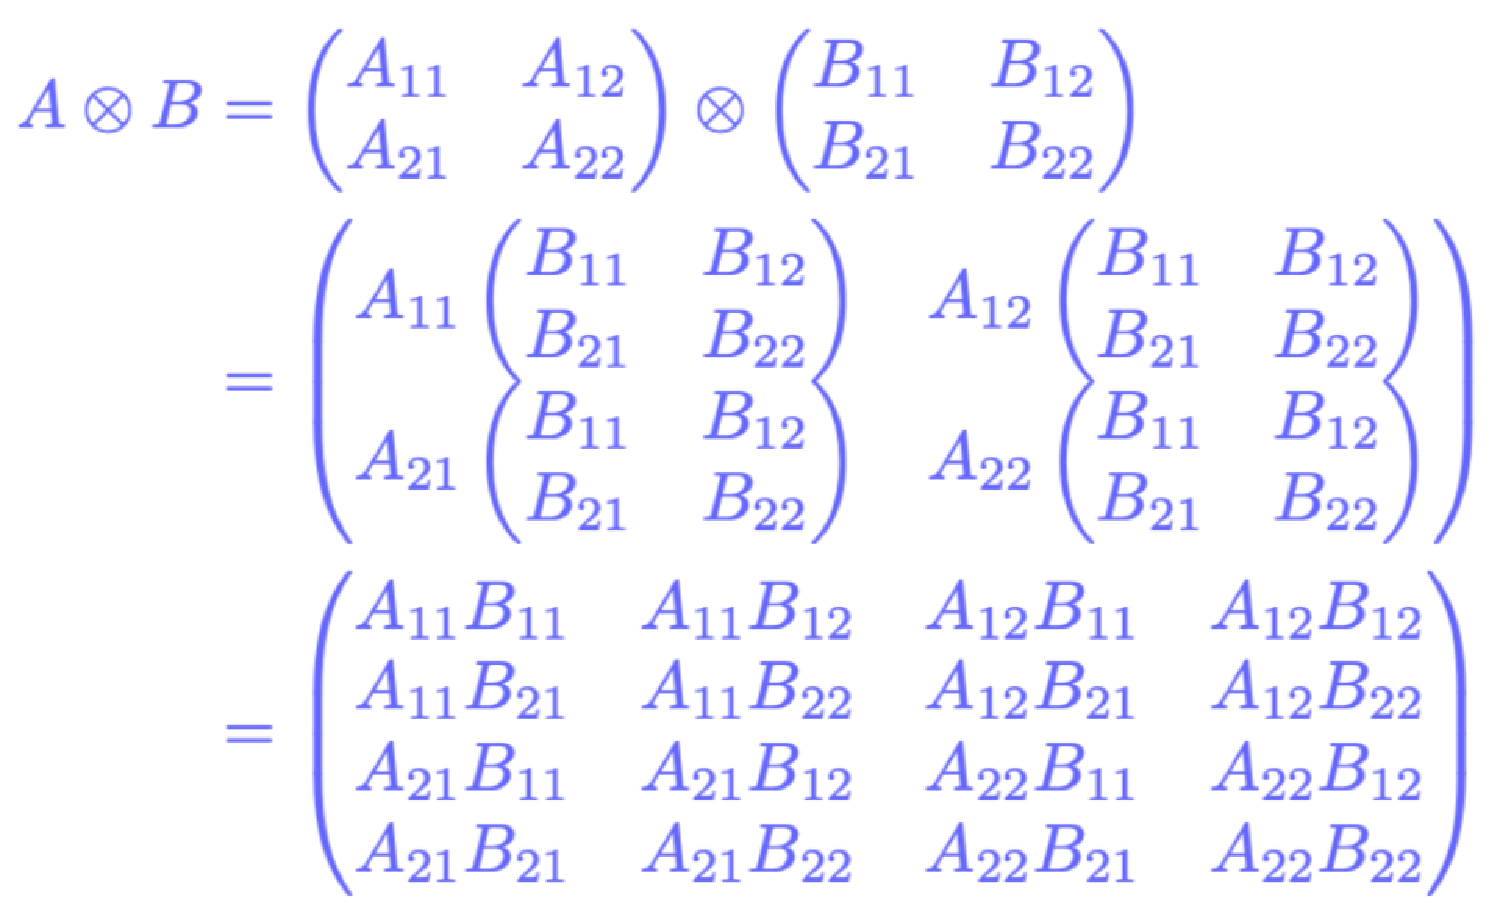
\includegraphics[width=0.8\textwidth]{lesson2/matrix_tensor.pdf}
    
        \caption{Matrix tensor}
    
    \label{fig:tensor-unused}
\end{figure}
\fi
%%%%%%%%%% end no need


In the upper left, we have $A_{11}$ times the matrix representation of $B$. In the upper right square, we have the element $A_{12}$ times the whole matrix $B$. In the lower left, we have  $A_{21}$ times matrix $B$, and finally in the lower right $A_{22}$ times matrix $B$. If you multiply out the whole equation, you can see that you have to calculate many individual matrix elements, or you can see that it's way simpler to write an equation in Dirac notation.

As an example, consider an operation on two qubits, applying an $X$ to our first (left) qubit, while leaving the second (right) qubit alone. This would be written as
\begin{equation}
\begin{aligned}
(X \otimes I)|\psi\rangle &=X \otimes I(\alpha|00\rangle+\beta|01\rangle+\gamma|10\rangle+\delta|11\rangle) \\
&=\alpha|10\rangle+\beta|11\rangle+\gamma|00\rangle+\delta|01\rangle
\end{aligned}
\end{equation}
If we write out the tensor of the operators, we have
\begin{equation}
(X \otimes I)=\left(\begin{array}{ll}
0 & 1 \\
1 & 0
\end{array}\right) \otimes\left(\begin{array}{ll}
1 & 0 \\
0 & 1
\end{array}\right)=\left(\begin{array}{llll}
0 & 0 & 1 & 0 \\
0 & 0 & 0 & 1 \\
1 & 0 & 0 & 0 \\
0 & 1 & 0 & 0
\end{array}\right).
\end{equation}

We can also see how to distribute independent operations. If we want to apply the operator $A$ to the state $\ket{a}$ and the operator $B$ to the state $\ket{b}$, we can apply the tensor conveniently before or after applying the operators to the states,
%We write the A tensor product B, operating on the ket "a" tensor product with "b", can be written as A- matrix A applied to ket a tensor product matrix B acting on ket b. 
\begin{equation}
(A \otimes B)|a\rangle \otimes|b\rangle=A|a\rangle \otimes B|b\rangle.
\end{equation}

Note that, unlike ordinary matrix multiplication, two matrices being tensored do not have to have a dimension in common. They can be any size. If $A$ is an $l\times m$ matrix and $B$ is an $n \times p$ matrix, the result will be an $ln \times mp$ matrix.

A note on notation: when tensoring kets, we can leave out the $\otimes$ symbol and just write $\ket{a}\ket{b}$ with the same meaning as $\ket{a}\otimes\ket{b}$. We cannot do the same with matrices, however, as that would be ambiguous with ordinary matrix multiplication.

Finally, by now you have probably recognized that one of the great advantages of the Dirac notation is its compactness. Two qubits can have four possible states, three qubits can have eight possible states, and so on; for $n$ qubits, the state vector is $2^n$ elements long when written out. But most of the time, we don't need to write out the entire state.  You have seen that the individual basis states are more compactly written, such as writing $\ket{00}$ instead of the whole four-element vector, let alone writing out the whole sixteen elements of the four-qubit state $\ket{0000}$. But more generally, even when dealing with an arbitrary state $\ket{\psi}$, we only need to write out the \emph{nonzero} elements, allowing us to ignore the zero elements.  Thus, a four-qubit superposition of the all-zeroes and all-ones states only requires us to write $\ket{\psi} = (\ket{0000} + \ket{1111})/\sqrt{2}$, saving our hands, our pens, and ultimately being easier cognitively as well~\footnote{If you are familiar with the execution of matrix math in high-performance computing, the Dirac and tensor notations are equivalent to a \emph{sparse representation}, keeping a list of nonzero elements instead of all of them.}.

\if0
$\left(\begin{array}{ll}
1 & 0 \\
0 & 1
\end{array}\right)$

$\left(\begin{array}{ll}
0 & 1 \\
1 & 0
\end{array}\right)$
\fi

\newpage
\begin{exercises}
\exer{Consider the following quantum state:}
\begin{equation*}
\ket{\psi} = \frac{\sqrt{3}}{2}\ket{0} + \frac{1}{2}\ket{1}
\end{equation*}
\subexer{Find the probability of measuring a zero.}
\subexer{Find the probability of measuring a one.}
\exer{Write out the vectors corresponding to the following tensor products. Confirm that the vectors remain normalized. Note that the order of writing the qubits matters, but the order of taking the products does not.} \subexer{$\ket{+}\otimes \ket{1}$.}
\subexer{$\ket{1}\otimes \ket{+}$.}
\subexer{$\ket{+}\otimes \ket{+}$.}
\subexer{$\ket{-}\otimes \ket{+}$.}
\subexer{$\ket{+}\otimes \ket{-}$.}
\subexer{$\ket{-}\otimes \ket{-}$.}
\subexer{$\ket{0}\otimes \ket{0} \otimes\ket{0}$.}
\subexer{$\ket{0}\otimes \ket{0} \otimes\ket{1}$.}
\subexer{$\ket{0}\otimes \ket{1} \otimes\ket{0}$.}
\subexer{$\ket{1}\otimes \ket{0} \otimes\ket{0}$.}
\subexer{$\ket{1}\otimes \ket{1} \otimes\ket{1}$.}
\subexer{$\ket{1}\otimes \ket{+} \otimes\ket{0}$.}

\exer{Write out the matrices corresponding to the following tensor products.} \subexer{$X\otimes X$.}
\subexer{$Z\otimes Z$.}
\subexer{$I\otimes X$.}
\subexer{$I\otimes Z$.}
\subexer{$X\otimes Z$.}
\subexer{$Z\otimes X$.}

\exer{Find the expectation value $\langle Z\rangle$ for the following single-qubit states.}
\subexer{$\ket{0}$}
\subexer{$\ket{1}$}
\subexer{$\ket{+}$}
\subexer{$\ket{-}$}
\subexer{$\frac{\sqrt{3}}{2}\ket{0} + \frac{1}{2}\ket{1}$}

\exer{Since we can find the expectation value of $Z$, you might suspect that we can do the same for $X$. Find the expectation value $\langle X\rangle$ for the following single-qubit states.}
\subexer{$\ket{0}$}
\subexer{$\ket{1}$}
\subexer{$\ket{+}$}
\subexer{$\ket{-}$}
\subexer{$\frac{\sqrt{3}}{2}\ket{0} + \frac{1}{2}\ket{1}$}

\exer{We said above that the Hadamard gate is not just a y-axis rotation.  To explore this further, calculate the following. \\
Use $\ket{\lambda_{+}} = \frac{\sqrt{2 + \sqrt{2}}}{2}\ket{0}+\frac{1}{\sqrt{2(2 + \sqrt{2})}}\ket{1}$ and $\ket{\lambda_{-}}=\frac{\sqrt{2 - \sqrt{2}}}{2}\ket{0} - \frac{1}{\sqrt{2(2 - \sqrt{2})}}\ket{1}$.
\subexer{$H\ket{i}$}
\subexer{$R_Y(\pi/2)\ket{i}$}
\subexer{$R_Y(\pi)\ket{i}$}
\subexer{$H(\sqrt{3}\ket{0}+\ket{1})/\sqrt{2}$}
\subexer{$R_Y(\pi/2)(\sqrt{3}\ket{0}+\ket{1})/\sqrt{2}$}
\subexer{$R_Y(\pi)(\sqrt{3}\ket{0}+\ket{1})/\sqrt{2}$}
\subexer{$H\ket{\lambda_+}$}
\subexer{$H\ket{\lambda_-}$}
\subexer{$R_Y(\pi/2)\ket{\lambda_+}$}
\subexer{$R_Y(\pi/2)\ket{\lambda_-}$}
\subexer{$R_Y(\pi)\ket{\lambda_+}$}
\subexer{$R_Y(\pi)\ket{\lambda_-}$}
}

\exer{
\label{ex:dirac-notation-measurement}
Let's explore single-qubit measurement in more depth. This will come in handy when we explore entanglement swapping in Sec.~\ref{sec:12-3_reaching_for_distance}. Another way of expressing measurement is to use $\operatorname{Prob}(i) = \bra{\psi}M_i\ket{\psi}$, where $\{M_i\}$ corresponds to the set of outcomes of our measurement operation. Each $M_i$ is written as an operator, $M_i = \ketbra{\psi_i}{\psi_i}$, and assuming there are two outcomes to the operation, $\pm 1$, then we have $M_{+1} = \ketbra{0}{0}$ and $M_{-1} = \ketbra{1}{1}$. Sometimes, we will write $M_{+1}^Z$ or $\Pi_{+1}^Z$ for measurement in the $Z$ basis, or even just $Z$.
\subexer{
Show that $\bra{\psi}M_i\ket{\psi}$ gives $|\alpha|^2$ and $|\beta|^2$ for \ket{0} and \ket{1}.
}
\subexer{
Find the set of operators $\{M_i\}$ when measuring in the $X$ basis. Show that they produce the same probabilities as Eq.~\ref{eq:plus-measurement} and \ref{eq:minus-measurement}.
}
\subexer{One way to find the post-measurement state of a state is
$$\ket{\psi'} = \frac{M_i\ket{\psi}}{\sqrt{\bra{\psi} M_i\ket{\psi}}}$$ when the outcome is $i$. Show that this gives exactly \ket{0} or \ket{1} when measuring in the computational basis, when $\ket{\psi} = \alpha\ket{0}+\beta\ket{1}$, for any value of $\alpha$ and $\beta$.
}
% \subexer{Show that $\bra{\psi} M_i\ket{\psi} = \bra{\psi}M_i^\dagger M_i \ket{\psi}$ for the measurement operations we have discussed so far. Identify any mathematical constraints on this equality holding. (Hint: this exercise is easy when you regroup bras and kets in the Dirac notation.)}
}
\end{exercises}

